%%% model definitions %%%

\begin{figure}[ht]
    \begin{subfigure}{\textwidth}
      \centering
      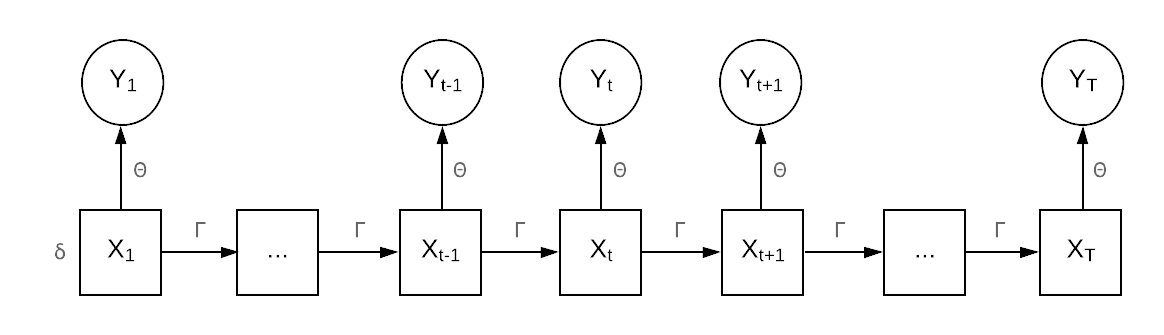
\includegraphics[width=4in]{../Plots/HMM.png}  
      \caption{Hidden Markov Model (\textbf{HMM})}
      \label{fig:HMM}
    \end{subfigure}
    %
    \newline
    %
    \begin{subfigure}{\textwidth}
      \centering
      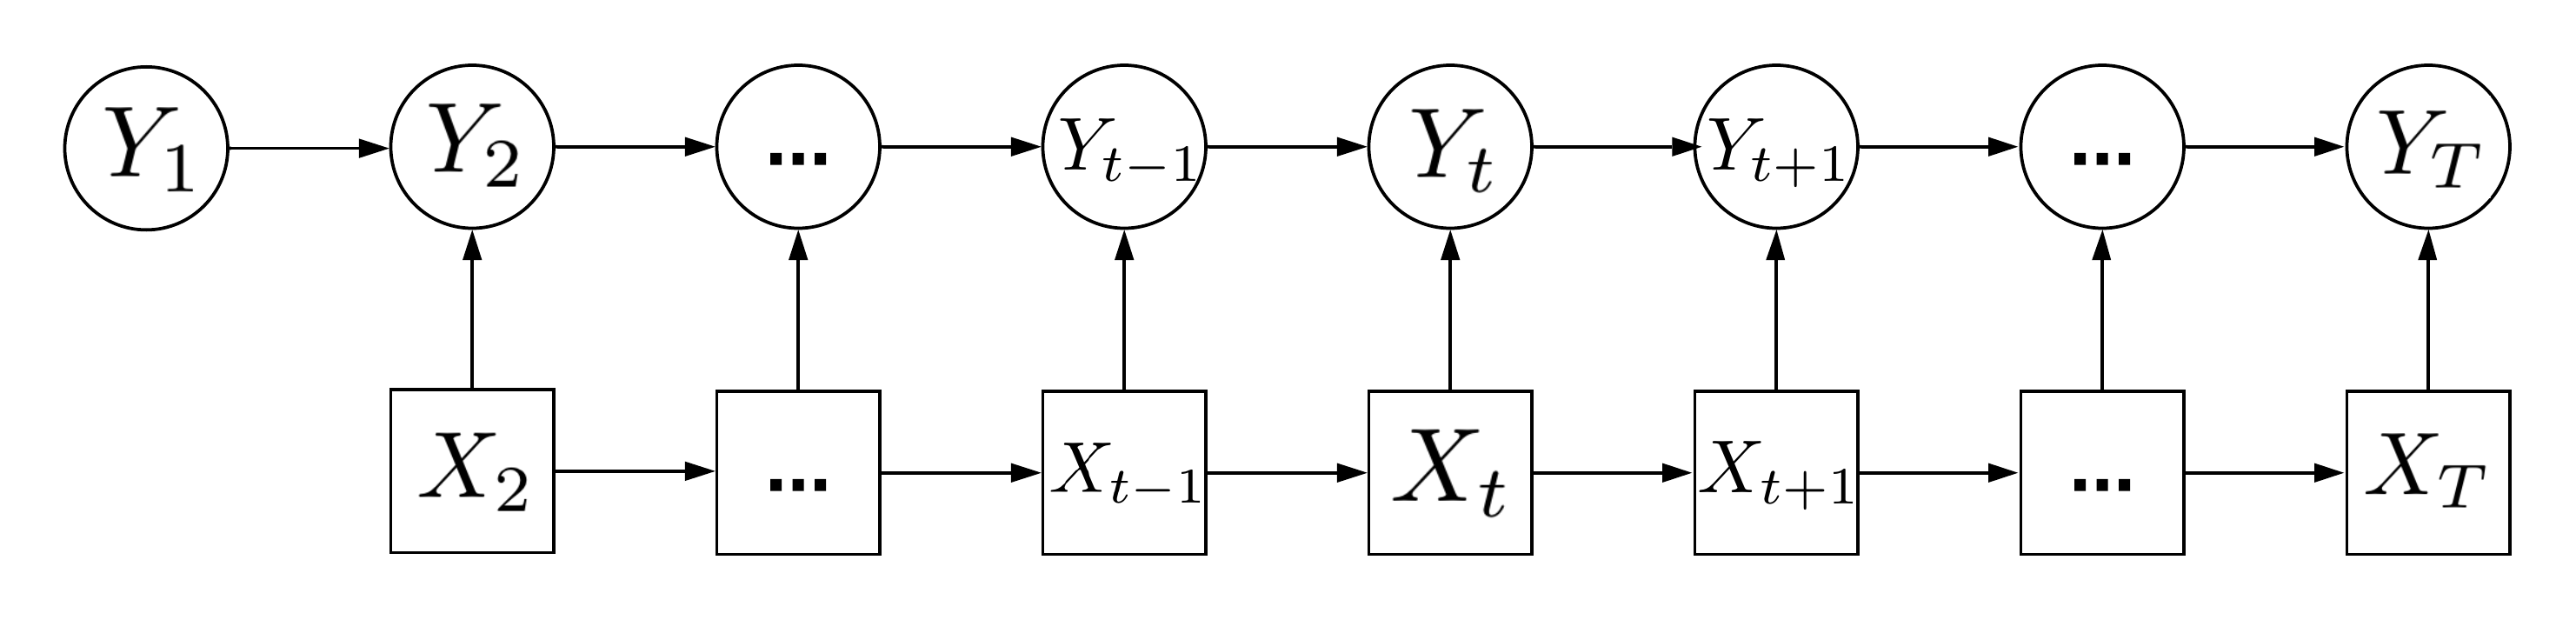
\includegraphics[width=4in]{../Plots/CarHMM.png}  
      \caption{Conditionally Auto-regressive HMM (\textbf{CarHMM})}
      \label{fig:CarHMM}
    \end{subfigure}
    %
    \newline
    %
    \begin{subfigure}{\textwidth}
      \centering
      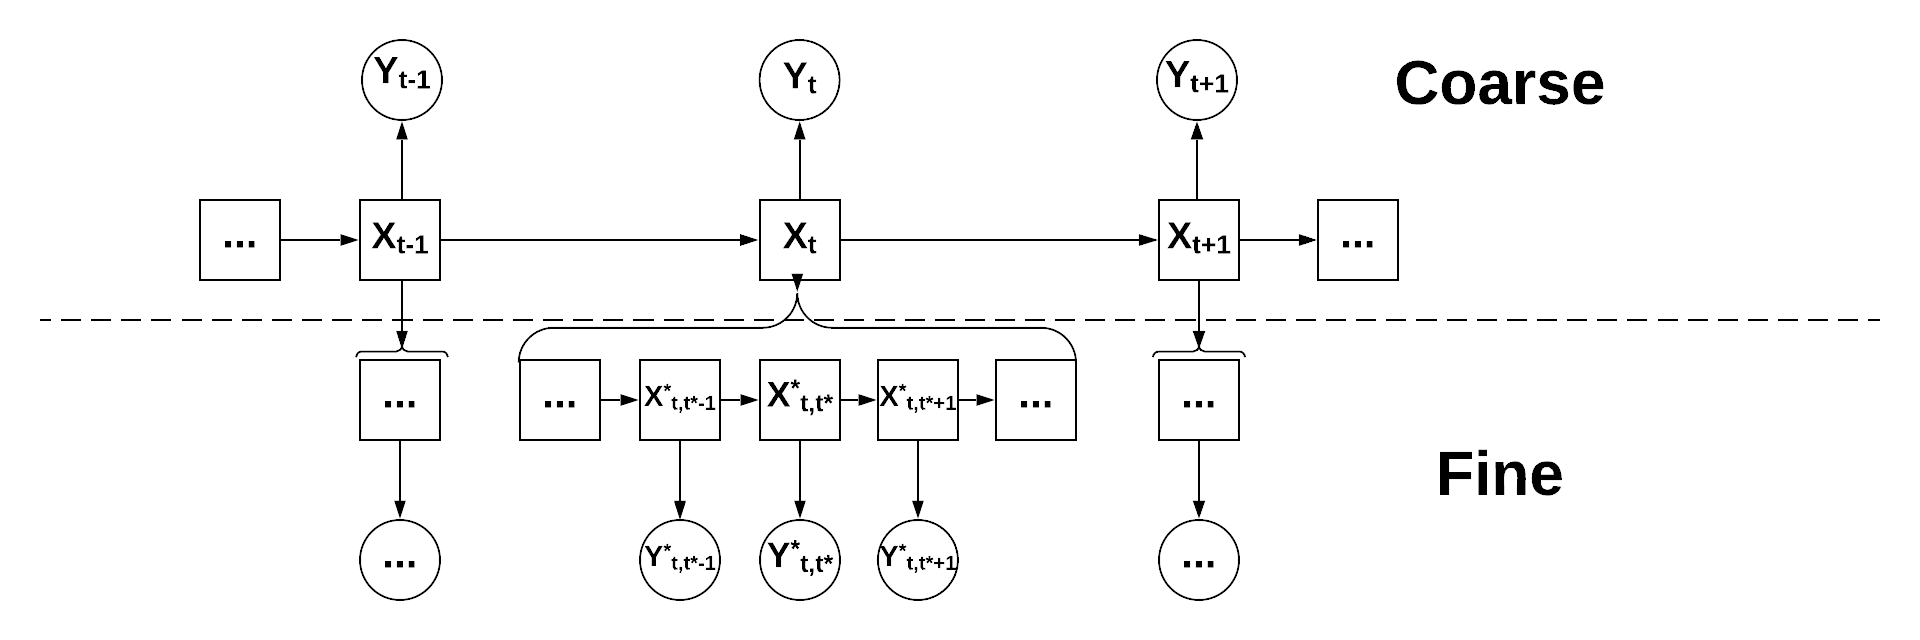
\includegraphics[width=4in]{../Plots/HHMM.png}  
      \caption{Hierarchical HMM (\textbf{HHMM})}
      \label{fig:HHMM}
    \end{subfigure}
    %
    \newline
    %
    \begin{subfigure}{\textwidth}
      \centering
      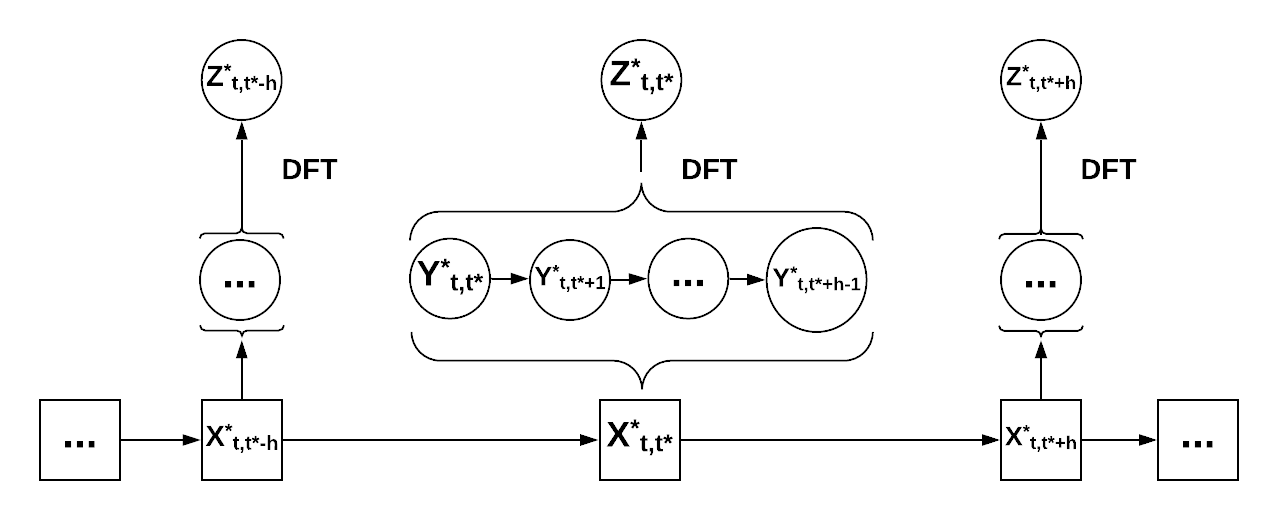
\includegraphics[width=4in]{../Plots/HMM-DFT.png}  
      \caption{HMM with Discrete Fourier Transform (\textbf{HMM-DFT})}
      \label{fig:HMM-DFT}
    \end{subfigure}
    \caption{Graphical representations of HMM models}
    \label{fig:graphical_models}
\end{figure}

%%% simulation study %%%

\begin{figure}[ht]
	\centering
	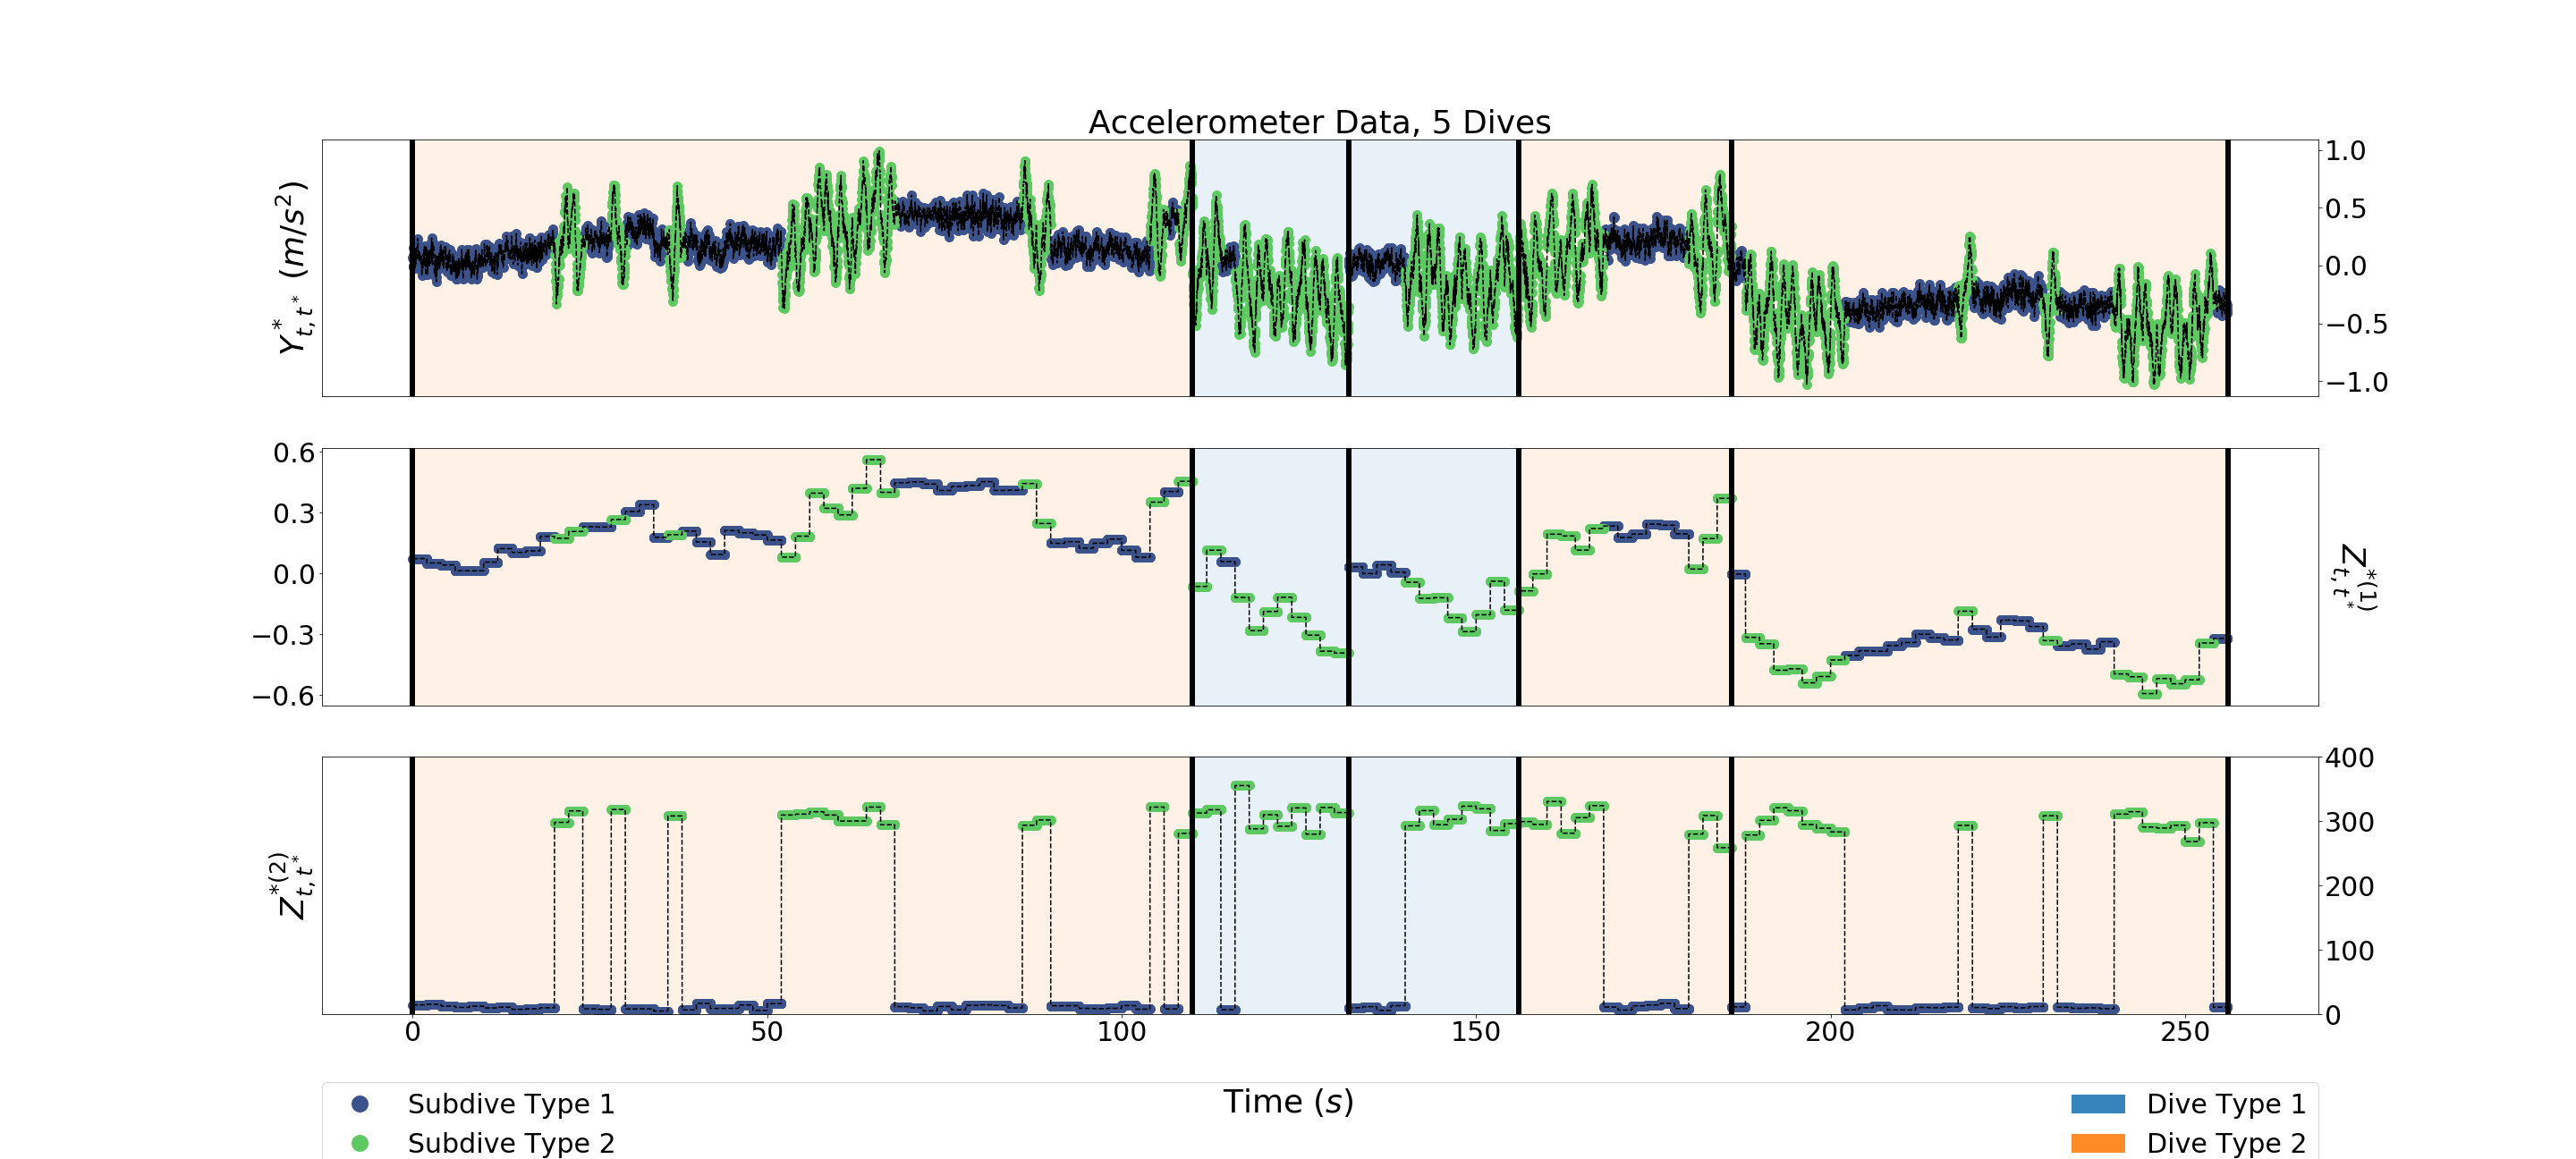
\includegraphics[width=5in]{../Plots/sim_data.png}
	\caption{Simulated acceleration data for one dive. The color of the line corresponds to the true fine-scale state of the sub-dive process, while the color of the background corresponds to the true dive type of the simulated whale.}
	\label{fig:sim_data}
\end{figure}

\begin{figure}[ht]
	\centering
	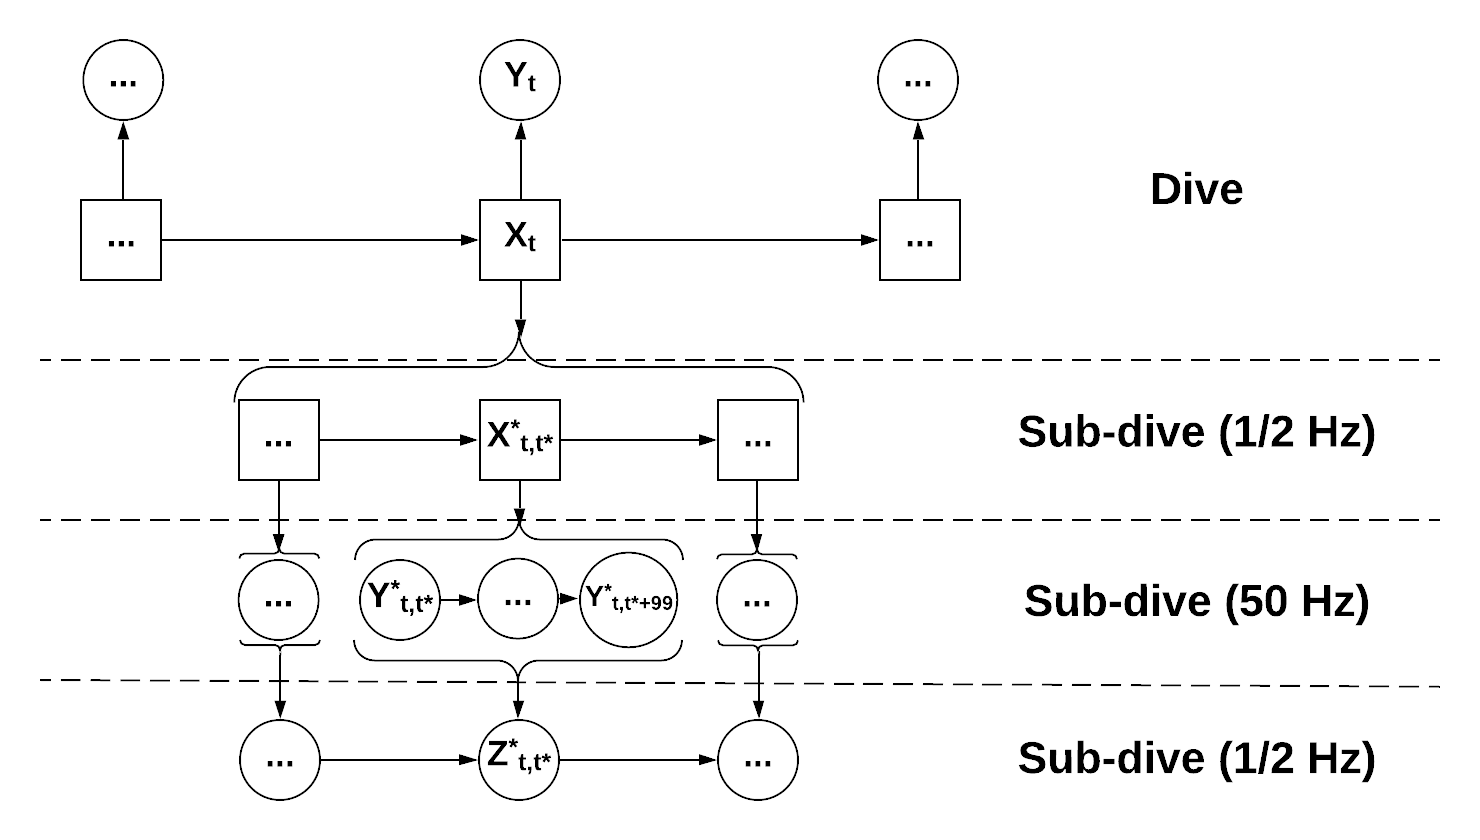
\includegraphics[width=5in]{../Plots/CarHHMM-DFT.png}
	\caption{Graphical representation the model used in the simulation and case study.}
	\label{fig:CarHHMM-DFT}
\end{figure}

\begin{figure}[ht]
    \centering
    \begin{subfigure}[t]{1.0\textwidth}
        \centering
        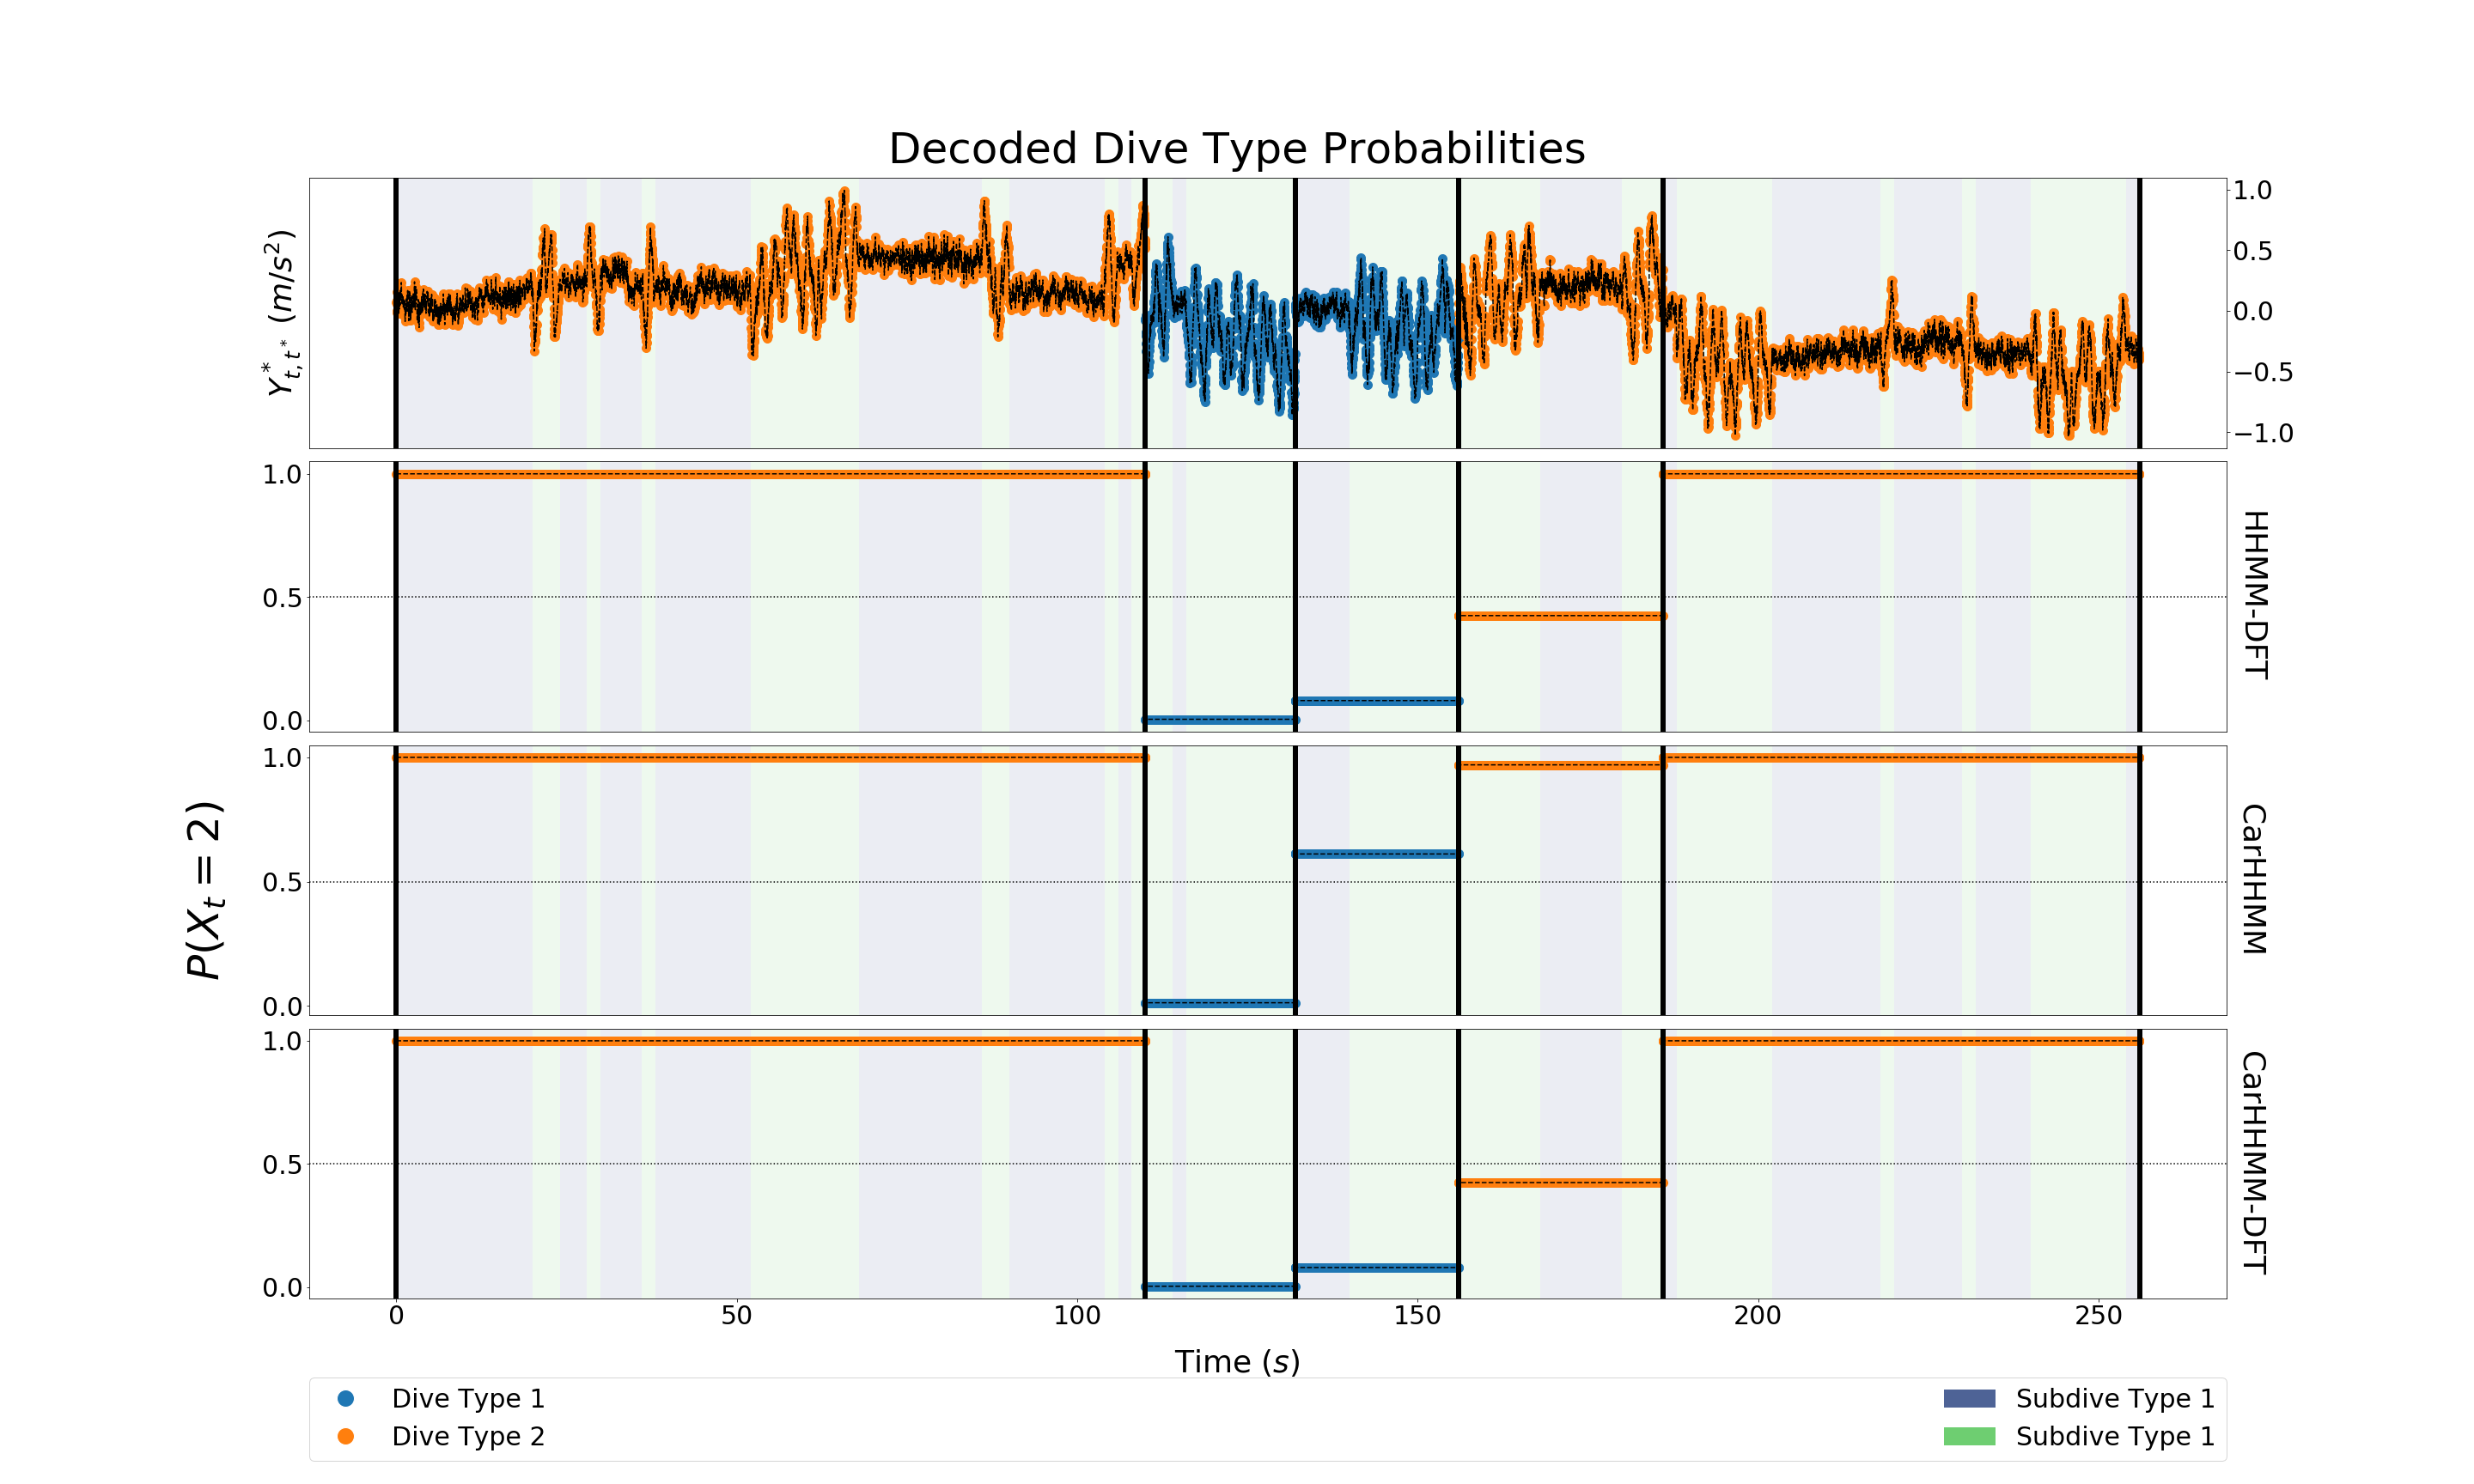
\includegraphics[width=5in]{Plots/Posterior_Coarse_States.png}
        \caption{Coarse-scale hidden process}
    \end{subfigure}
    \newline
    \begin{subfigure}[t]{1.0\textwidth}
        \centering
        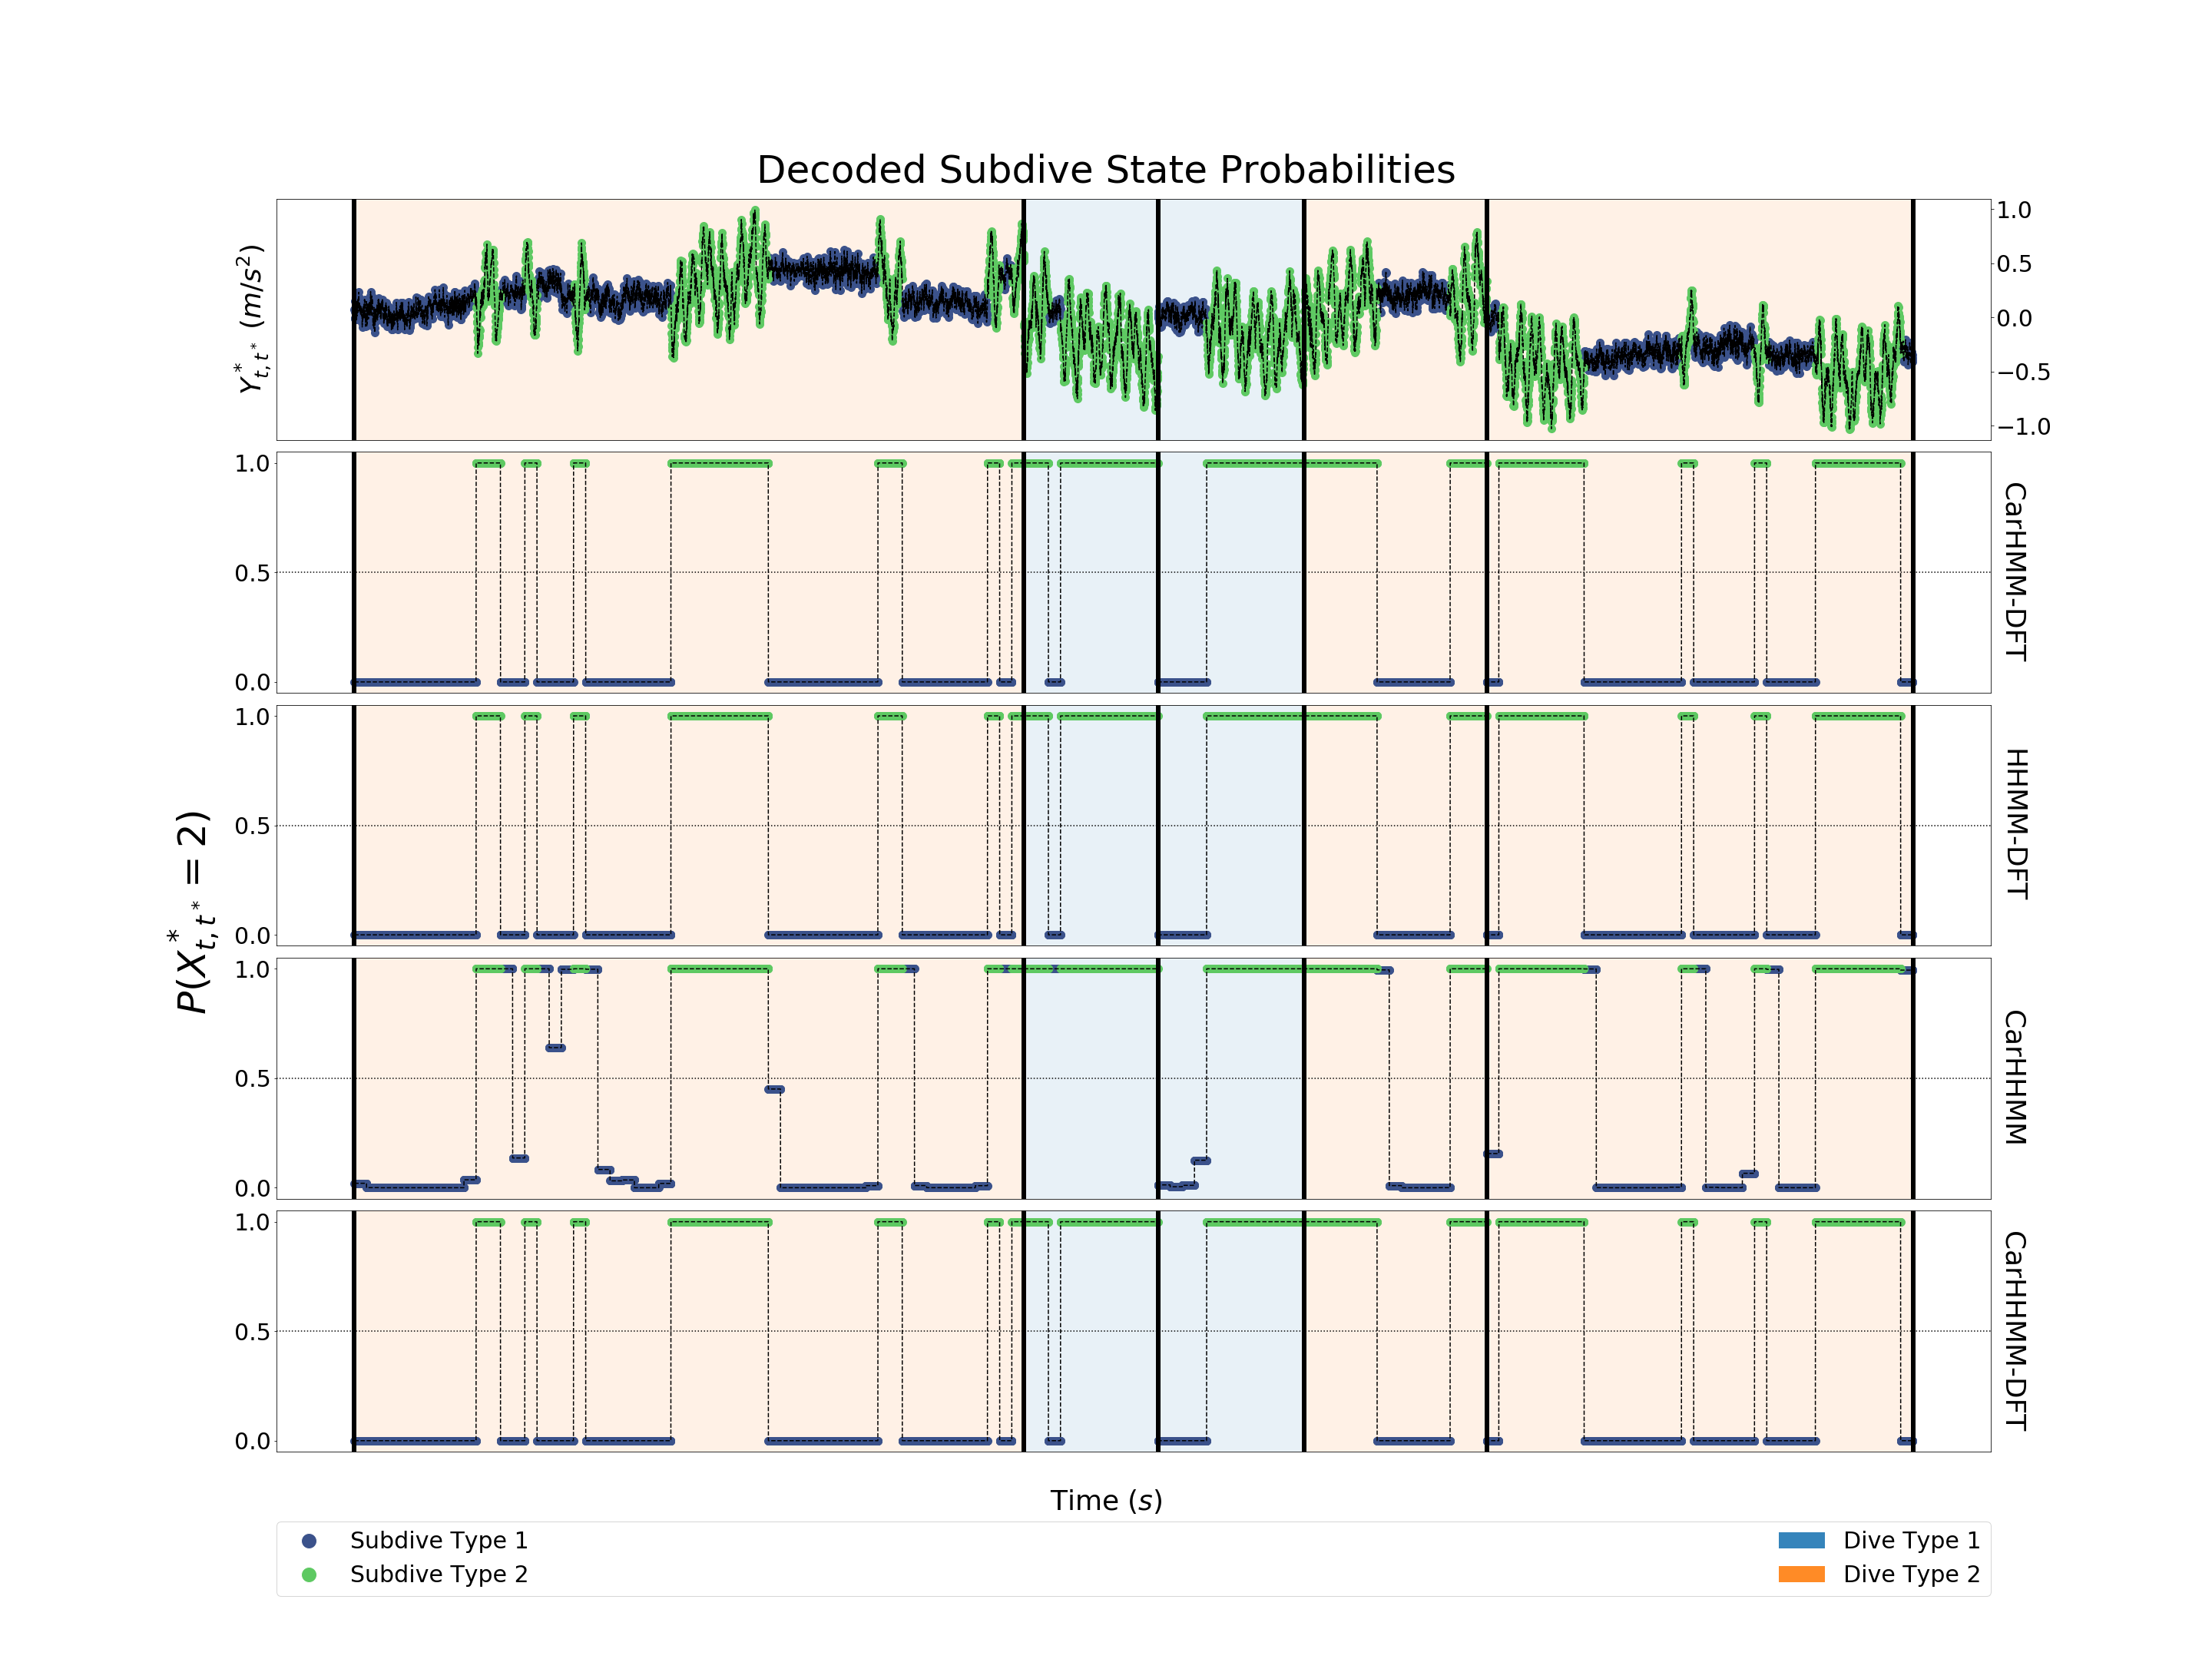
\includegraphics[width=5in]{Plots/Posterior_Fine_States.png}
        \caption{Fine-scale hidden process}
    \end{subfigure}
	\caption{Decoded state probabilities of each model}
	\label{fig:acc}
\end{figure}

\begin{figure}[ht]
    \centering
    \begin{subfigure}[t]{0.4\textwidth}
        \centering
        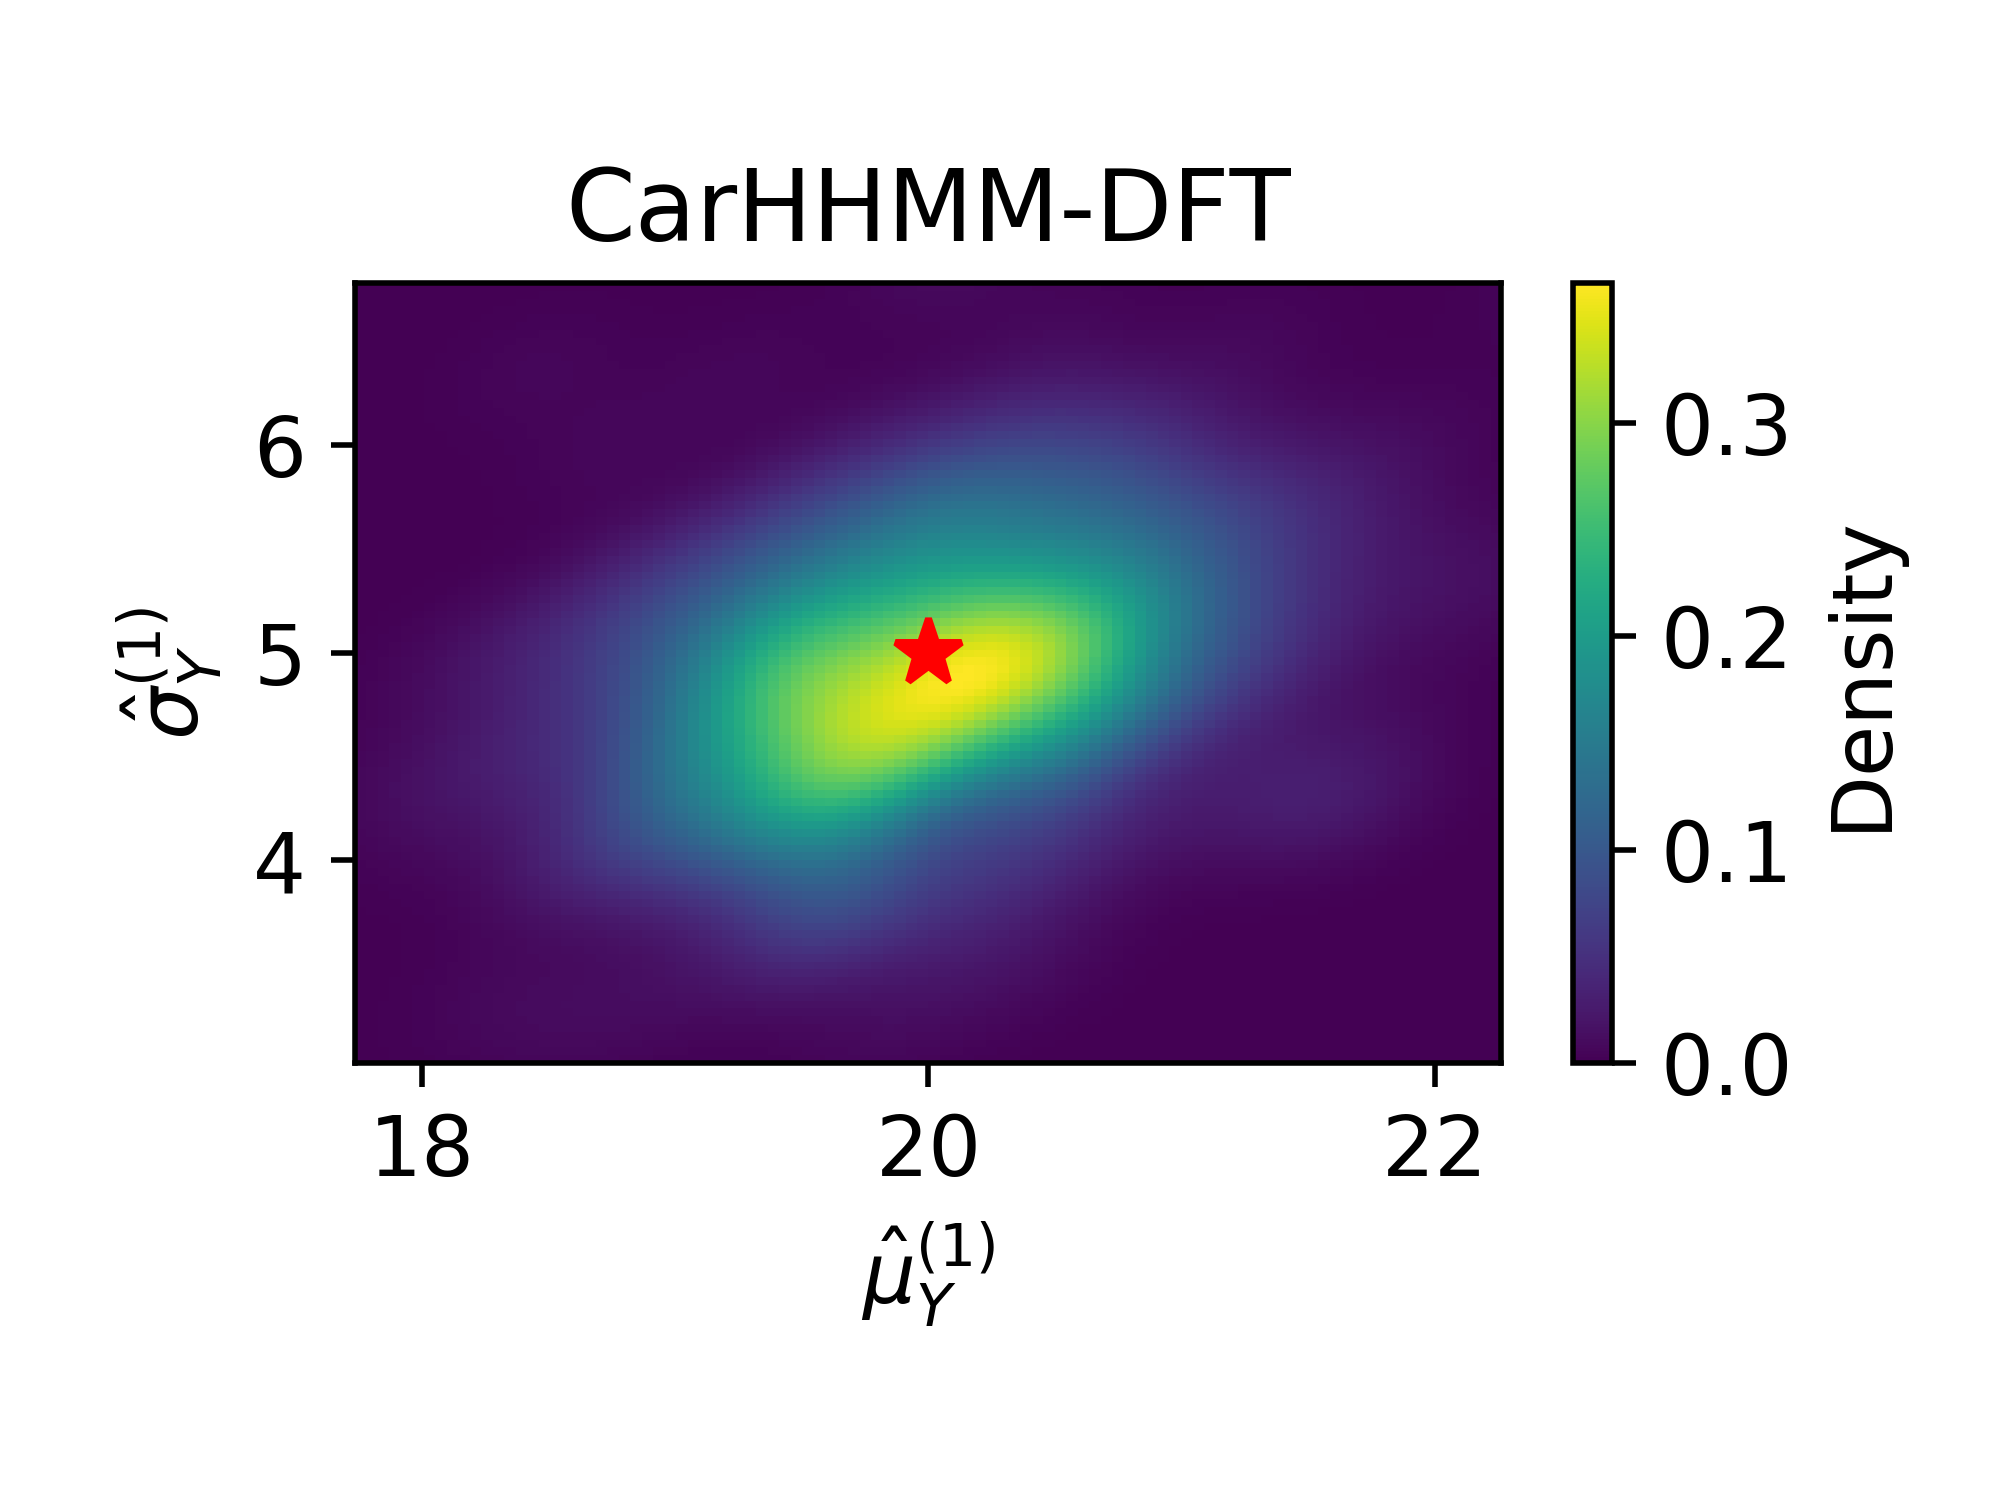
\includegraphics[width=2in]{../Plots/hhmm_FV_MLE_density_dive_duration_-1_0.png}
        \caption{Dive Type 1}
    \end{subfigure}
    %
    \begin{subfigure}[t]{0.4\textwidth}
        \centering
        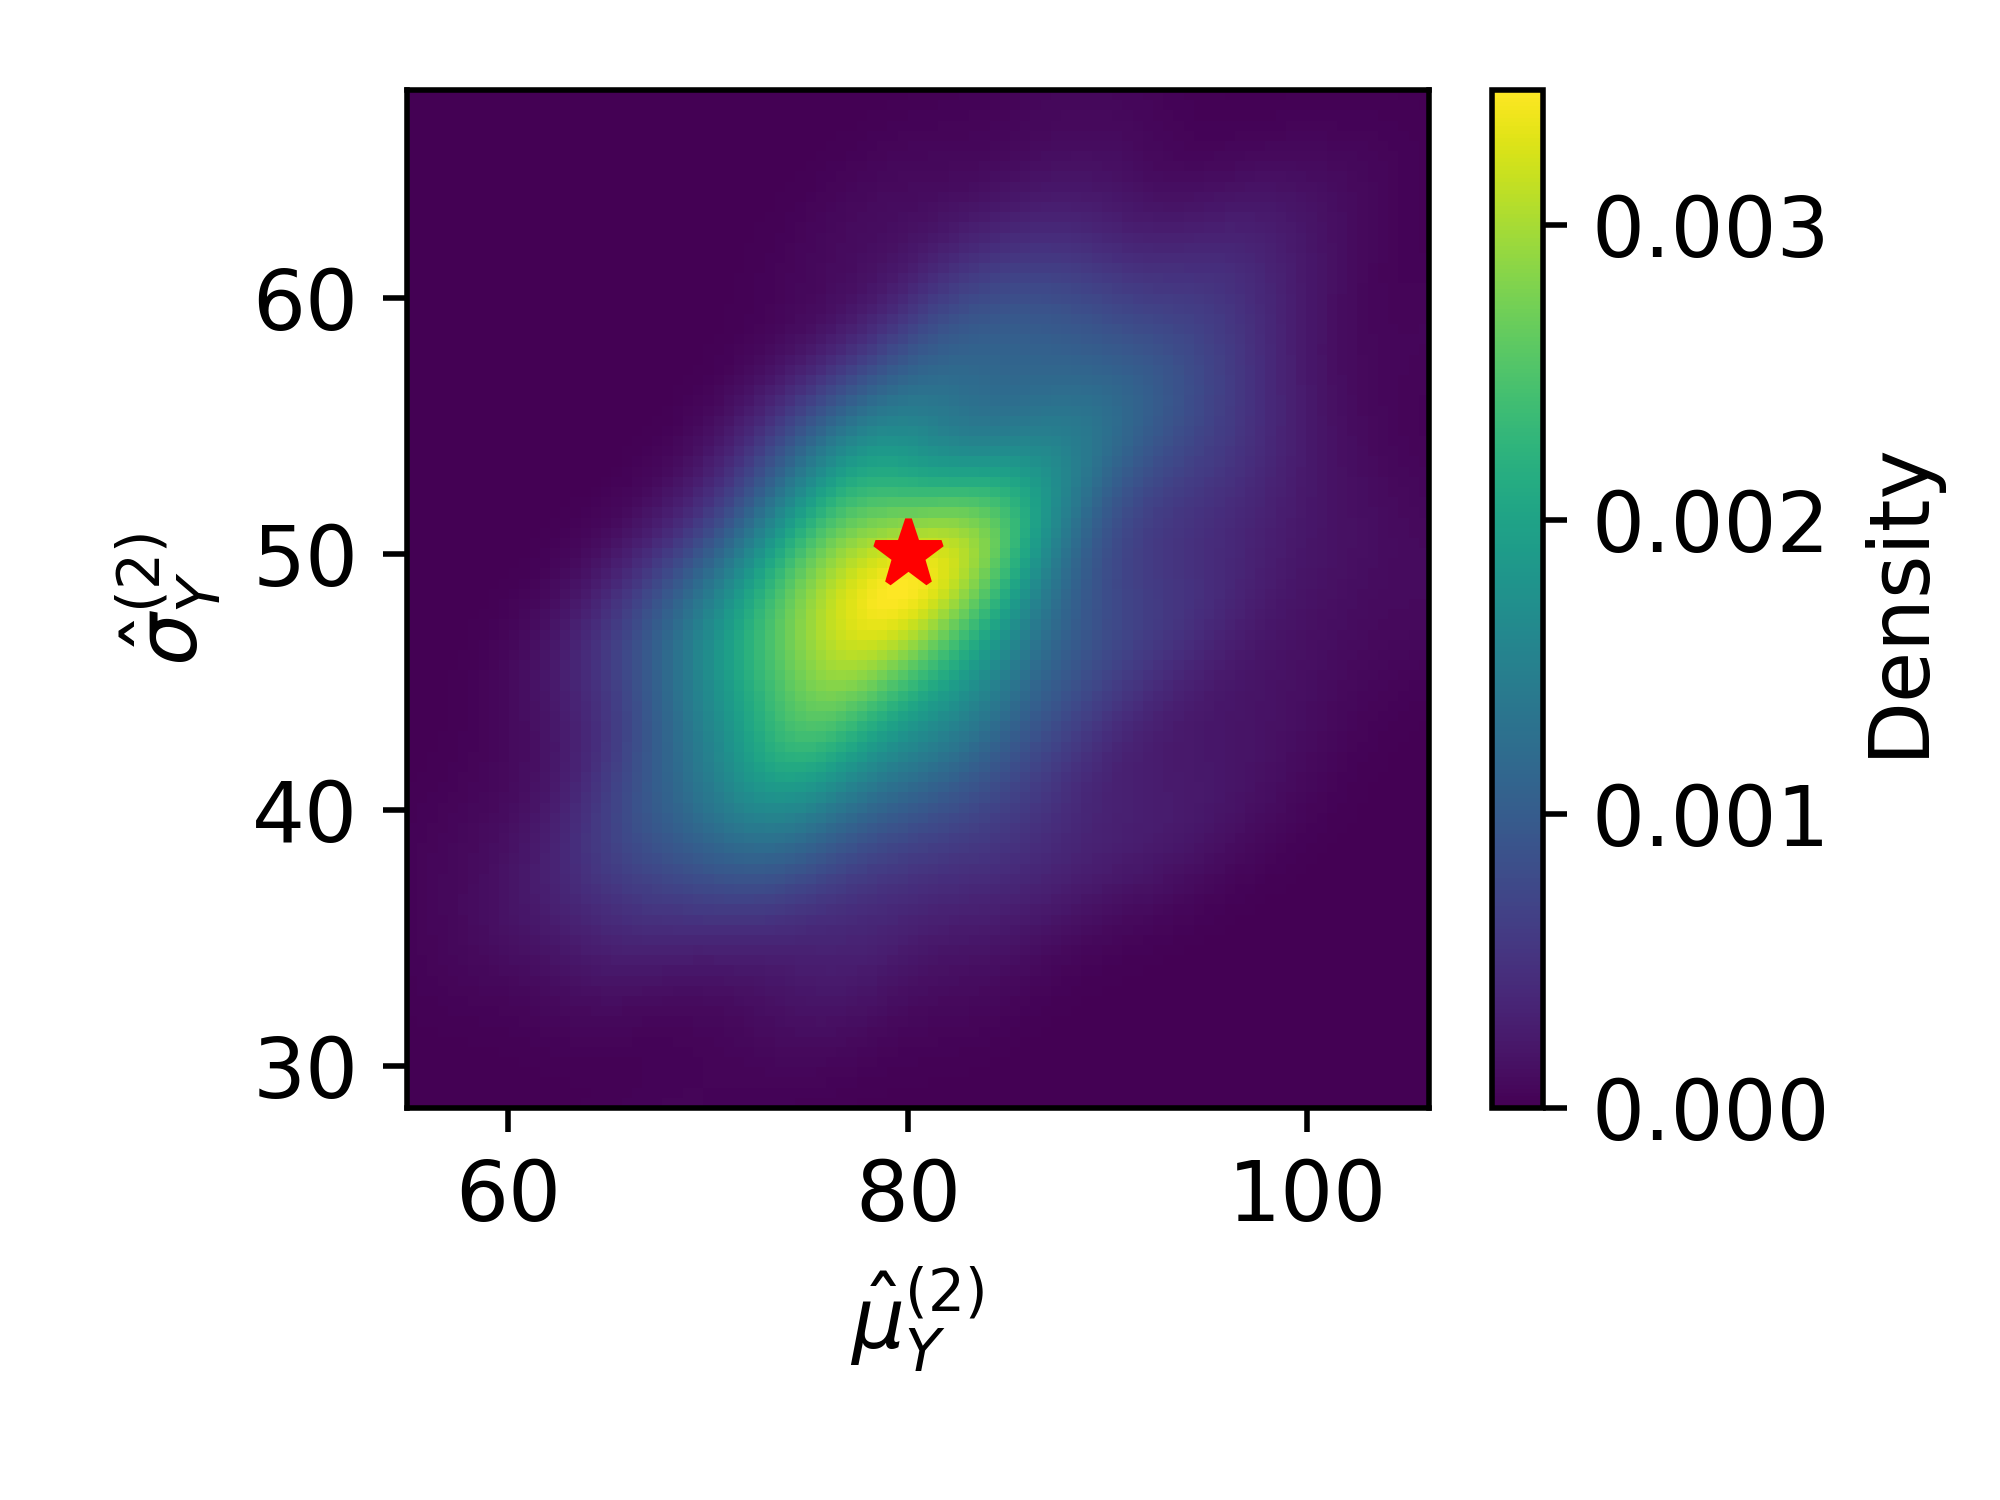
\includegraphics[width=2in]{../Plots/hhmm_FV_MLE_density_dive_duration_-1_1.png}
        \caption{Dive Type 2}
    \end{subfigure}
	\caption{KDE plot of $\hat \mu$ and $\hat \sigma$ for the dive duration emission distribution for the CarHMM.}
	\label{fig:MLE_dist}
\end{figure}

%%% Accuracy %%%

\begin{table}
\centering
\caption{Accuracies and run times for all models. All reported values are averages, and $\pm$ refers to the standard deviation.}
\scalebox{0.8}{
\begin{tabular}{ccccccc}
Model                      & \multicolumn{1}{c}{Training Time (Minutes)} & \multicolumn{1}{c}{Dive Type} & \multicolumn{1}{c}{Subdive Type} & \multicolumn{1}{c}{Dive Accuracy} & \multicolumn{1}{c}{Subdive Accuracy}  \\ \hline
\multirow{5}{*}{CarHMM-DFT}& \multirow{5}{*}{$15.74 \pm 2.46$}   & Both                          & Both                             & -------------                     & $1.00 \pm 0.00$                       \\
                           &                                    & 1                             & 1                                & \multirow{2}{*}{-------------}    & $1.00 \pm 0.00$                       \\ 
                           &                                    & 1                             & 2                                &                                   & $1.00 \pm 0.00$                       \\ 
                           &                                    & 2                             & 1                                & \multirow{2}{*}{-------------}    & $1.00 \pm 0.00$                       \\ 
                           &                                    & 2                             & 2                                &                                   & $1.00 \pm 0.00$                       \\ \hline 
\multirow{5}{*}{HHMM-DFT}  & \multirow{5}{*}{$82.43 \pm 11.48$}   & Both                          & Both                             & $0.94 \pm 0.02$                   & $1.00 \pm 0.00$                       \\
                           &                                    & 1                             & 1                                & \multirow{2}{*}{$0.94\pm0.03$}    & $1.00 \pm 0.00$                       \\ 
                           &                                    & 1                             & 2                                &                                   & $1.00 \pm 0.00$                       \\ 
                           &                                    & 2                             & 1                                & \multirow{2}{*}{$0.94\pm0.03$}    & $1.00 \pm 0.00$                       \\ 
                           &                                    & 2                             & 2                                &                                   & $1.00 \pm 0.00$                       \\ \hline
\multirow{5}{*}{CarHHMM}   & \multirow{5}{*}{$70.85 \pm 15.89$}   & Both                          & Both                             & $0.91 \pm 0.03$                   & $0.89 \pm 0.02$                       \\
                           &                                    & 1                             & 1                                & \multirow{2}{*}{$0.87\pm0.04$}    & $0.44 \pm 0.12$                       \\ 
                           &                                    & 1                             & 2                                &                                   & $1.00 \pm 0.00$                       \\ 
                           &                                    & 2                             & 1                                & \multirow{2}{*}{$0.95\pm0.03$}    & $0.81 \pm 0.04$                       \\ 
                           &                                    & 2                             & 2                                &                                   & $1.00 \pm 0.00$                       \\ \hline
\multirow{5}{*}{CarHHMM-DFT}& \multirow{5}{*}{$81.22 \pm 16.10$}   & Both                          & Both                             & $0.94 \pm 0.02$                   & $1.00 \pm 0.00$                       \\
                           &                                    & 1                             & 1                                & \multirow{2}{*}{$0.94\pm0.03$}    & $1.00 \pm 0.00$                       \\ 
                           &                                    & 1                             & 2                                &                                   & $1.00 \pm 0.00$                       \\ 
                           &                                    & 2                             & 1                                & \multirow{2}{*}{$0.94\pm0.03$}    & $1.00 \pm 0.00$                       \\ 
                           &                                    & 2                             & 2                                &                                   & $1.00 \pm 0.00$                       \\ \hline
\end{tabular}
}
\label{table:accuracy}
\end{table}

%%% dive duration %%%

\begin{table}
\centering
\caption{Estimates and standard errors of parameters for dive duration distribution for all four models. All reported values are averages, except for the Fisher observed standard error, which are medians. $\pm$ refers to the IQR.}
\scalebox{0.9}{
\begin{tabular}{ccccccc}
Model                      & \multicolumn{1}{c}{Parameter} & \multicolumn{1}{c}{Dive Type} & \multicolumn{1}{c}{Estimate} & \multicolumn{1}{c}{Bias} & \multicolumn{1}{c}{Empirical SE} & \multicolumn{1}{c}{Observed Fischer SE}           \\ \hline
\multirow{4}{*}{CarHMM-DFT}& \multirow{2}{*}{$\mu$}        & 1                             & $49.72$                         & $-0.28$                     & $4.78$                             & $2.47 \pm 0.34$                             \\
                           &                               & ---                           & ---                            & ---                        & ---                                & ---                                         \\
                           & \multirow{2}{*}{$\sigma$}     & 1                             & $39.00$                         & $-7.51$                     & $5.05$                             & $2.50 \pm 0.40$                             \\
                           &                               & ---                           & ---                            & ---                        & ---                                & ---                                         \\ \hline
\multirow{4}{*}{HHMM-DFT}  & \multirow{2}{*}{$\mu$}        & 1                             & $19.99$                         & $-0.01$                     & $0.75$                             & $0.69 \pm 0.11$                             \\
                           &                               & 2                             & $79.85$                         & $-0.15$                     & $8.05$                             & $5.85 \pm 1.10$                             \\
                           & \multirow{2}{*}{$\sigma$}     & 1                             & $4.90$                         & $-0.10$                     & $0.61$                             & $0.53 \pm 0.10$                             \\
                           &                               & 2                             & $48.74$                         & $-1.26$                     & $6.50$                             & $5.15 \pm 1.02$                             \\ \hline
\multirow{4}{*}{CarHHMM}   & \multirow{2}{*}{$\mu$}        & 1                             & $19.91$                         & $-0.09$                     & $0.77$                             & $0.71 \pm 0.12$                             \\
                           &                               & 2                             & $75.80$                         & $-4.20$                     & $7.72$                             & $5.32 \pm 0.98$                             \\
                           & \multirow{2}{*}{$\sigma$}     & 1                             & $4.73$                         & $-0.27$                     & $0.59$                             & $0.55 \pm 0.10$                             \\
                           &                               & 2                             & $49.48$                         & $-0.52$                     & $6.26$                             & $4.79 \pm 0.93$                             \\ \hline
\multirow{4}{*}{CarHHMM-DFT}& \multirow{2}{*}{$\mu$}        & 1                             & $19.99$                         & $-0.01$                     & $0.75$                             & $0.69 \pm 0.12$                             \\
                           &                               & 2                             & $79.85$                         & $-0.15$                     & $8.05$                             & $5.85 \pm 1.10$                             \\
                           & \multirow{2}{*}{$\sigma$}     & 1                             & $4.90$                         & $-0.10$                     & $0.61$                             & $0.53 \pm 0.10$                             \\
                           &                               & 2                             & $48.74$                         & $-1.26$                     & $6.50$                             & $5.15 \pm 1.02$                             
\end{tabular}
}
\label{table:dive_duration}
\end{table}


%%% Acceleration %%%

\begin{table}
\centering
\caption{Estimates and standard errors of parameters for $Z^{*(1)}_{t,t^*}$ for all four models. All reported values are averages, except for the Fisher observed standard error, which are medians. $\pm$ refers to the IQR.}
\scalebox{0.7}{
\begin{tabular}{ccccccc}
Model                      & \multicolumn{1}{c}{Parameter} & \multicolumn{1}{c}{Subdive Type} & \multicolumn{1}{c}{Estimate} & \multicolumn{1}{c}{Bias} & \multicolumn{1}{c}{Empirical SE} & \multicolumn{1}{c}{Observed Fischer SE}        \\ \hline
\multirow{6}{*}{CarHMM-DFT}& \multirow{2}{*}{$\mu$}        & 1                             & $0.00$                         & $0.00$                     & $0.00$                             & $0.14 \pm 0.13$                             \\
                           &                               & 2                             & $0.00$                         & $0.00$                     & $0.01$                             & $0.06 \pm 0.02$                             \\
                           & \multirow{2}{*}{$\sigma$}     & 1                             & $0.05$                         & $-0.00$                     & $0.00$                             & $0.00 \pm 0.00$                             \\
                           &                               & 2                             & $0.10$                         & $-0.00$                     & $0.00$                             & $0.00 \pm 0.00$                             \\ 
                           & \multirow{2}{*}{$\phi$}       & 1                             & $0.99$                         & $-0.00$                     & $0.01$                             & $0.01 \pm 0.00$                             \\
                           &                               & 2                             & $0.95$                         & $-0.00$                     & $0.01$                             & $0.01 \pm 0.00$                             \\ \hline
\multirow{6}{*}{HHMM-DFT}  & \multirow{2}{*}{$\mu$}        & 1                             & $-0.01$                         & $-0.01$                     & $0.02$                             & $0.01 \pm 0.00$                             \\
                           &                               & 2                             & $-0.00$                         & $-0.00$                     & $0.02$                             & $0.01 \pm 0.00$                             \\
                           & \multirow{2}{*}{$\sigma$}     & 1                             & $0.25$                         & $0.20$                     & $0.04$                             & $0.00 \pm 0.00$                             \\
                           &                               & 2                             & $0.24$                         & $0.14$                     & $0.03$                             & $0.00 \pm 0.00$                             \\ 
                           & \multirow{2}{*}{$\phi$}       & 1                             & ------                         & ------                     & ------                             & ------                                      \\
                           &                               & 2                             & ------                         & ------                     & ------                             & ------                                      \\ \hline
\multirow{6}{*}{CarHHMM}   & \multirow{2}{*}{$\mu$}        & 1                             & $0.00$                         & $0.00$                     & $0.00$                             & $0.08 \pm 0.04$                             \\
                           &                               & 2                             & $-0.01$                         & $-0.01$                     & $0.01$                             & $0.01 \pm 0.00$                             \\
                           & \multirow{2}{*}{$\sigma$}     & 1                             & $0.05$                         & $0.00$                     & $0.04$                             & $0.00 \pm 0.00$                             \\
                           &                               & 2                             & $0.27$                         & $0.17$                     & $0.01$                             & $0.00 \pm 0.00$                             \\ 
                           & \multirow{2}{*}{$\phi$}       & 1                             & $0.97$                         & $-0.02$                     & $0.10$                             & $0.00 \pm 0.00$                             \\
                           &                               & 2                             & $0.49$                         & $-0.46$                     & $0.05$                             & $0.02 \pm 0.00$                             \\ \hline
\multirow{6}{*}{CarHHMM-DFT}& \multirow{2}{*}{$\mu$}        & 1                             & $0.00$                         & $0.00$                     & $0.00$                             & $0.13 \pm 0.12$                             \\
                           &                               & 2                             & $0.00$                         & $0.00$                     & $0.00$                             & $0.06 \pm 0.02$                             \\
                           & \multirow{2}{*}{$\sigma$}     & 1                             & $0.05$                         & $-0.00$                     & $0.00$                             & $0.00 \pm 0.00$                             \\
                           &                               & 2                             & $0.10$                         & $-0.00$                     & $0.00$                             & $0.00 \pm 0.00$                             \\ 
                           & \multirow{2}{*}{$\phi$}       & 1                             & $0.99$                         & $-0.00$                     & $0.01$                             & $0.01 \pm 0.00$                             \\
                           &                               & 2                             & $0.95$                         & $-0.00$                     & $0.01$                             & $0.01 \pm 0.00$                             \\ \hline
\end{tabular}
}
\label{table:acceleration}
\end{table}


%%% FoVeDBA %%%

\begin{table}
\centering
\caption{Estimates and standard errors of parameters for $Z^{*(2)}_{t,t^*}$ for all four models. All reported values are averages, except for the Fisher observed standard error, which are medians. $\pm$ refers to the IQR.}
\scalebox{0.8}{
\begin{tabular}{ccccccc}
Model                      & \multicolumn{1}{c}{Parameter} & \multicolumn{1}{c}{Subdive Type} & \multicolumn{1}{c}{Estimate} & \multicolumn{1}{c}{Bias} & \multicolumn{1}{c}{Empirical SE} & \multicolumn{1}{c}{Observed Fischer SE}        \\ \hline
\multirow{4}{*}{CarHMM-DFT}& \multirow{2}{*}{$\mu$}        & 1                             & $10.10$                         & $-0.00$                     & $0.09$                             & $0.08 \pm 0.01$                             \\
                           &                               & 2                             & $305.97$                         & $0.03$                     & $0.54$                             & $0.51 \pm 0.03$                             \\
                           & \multirow{2}{*}{$\sigma$}     & 1                             & $3.18$                         & $-0.00$                     & $0.07$                             & $0.06 \pm 0.01$                             \\
                           &                               & 2                             & $17.46$                         & $-0.03$                     & $0.37$                             & $0.36 \pm 0.02$                             \\ \hline
\multirow{4}{*}{HHMM-DFT}  & \multirow{2}{*}{$\mu$}        & 1                             & $10.10$                         & $-0.00$                     & $0.09$                             & $0.08 \pm 0.01$                             \\
                           &                               & 2                             & $305.97$                         & $0.03$                     & $0.54$                             & $0.51 \pm 0.03$                             \\
                           & \multirow{2}{*}{$\sigma$}     & 1                             & $3.18$                         & $-0.00$                     & $0.07$                             & $0.06 \pm 0.01$                             \\
                           &                               & 2                             & $17.46$                         & $-0.03$                     & $0.37$                             & $0.36 \pm 0.02$                             \\ \hline
\multirow{4}{*}{CarHHMM}   & \multirow{2}{*}{$\mu$}        & 1                             & ------                         & ------                     & ------                             & ------                                      \\
                           &                               & 2                             & ------                         & ------                     & ------                             & ------                                      \\
                           & \multirow{2}{*}{$\sigma$}     & 1                             & ------                         & ------                     & ------                             & ------                                      \\
                           &                               & 2                             & ------                         & ------                     & ------                             & ------                                      \\ \hline
\multirow{4}{*}{CarHHMM-DFT}& \multirow{2}{*}{$\mu$}        & 1                             & $10.10$                         & $-0.00$                     & $0.09$                             & $0.08 \pm 0.01$                             \\
                           &                               & 2                             & $305.97$                         & $0.03$                     & $0.54$                             & $0.51 \pm 0.03$                             \\
                           & \multirow{2}{*}{$\sigma$}     & 1                             & $3.18$                         & $-0.00$                     & $0.07$                             & $0.06 \pm 0.01$                             \\
                           &                               & 2                             & $17.46$                         & $-0.03$                     & $0.37$                             & $0.36 \pm 0.02$                             
\end{tabular}
}
\label{table:FoVeDBA}
\end{table}

% Gamma
\begin{table}[t]
\centering
\caption{Estimates and standard errors of $\Gamma$ and $\Gamma^*$ for all four models. All reported values are averages except for the observed fisher SE, which is a median. $\pm$ refers to the IQR.}
\scalebox{0.7}{
\begin{tabular}{ccccccc}
Model                        & \multicolumn{1}{c}{Parameter} & \multicolumn{1}{c}{Estimate}   & \multicolumn{1}{c}{Bias} & \multicolumn{1}{c}{Empirical SE} & \multicolumn{1}{c}{Observed Fischer SE}     \\ \hline
\multirow{6}{*}{HHMM-DFT}    & $\Gamma_{12}$                 & $0.50$                         & $-0.00$                   & $0.03$                           & $0.08 \pm 0.01$                             \\
                             & $\Gamma_{21}$                 & $0.50$                         & $-0.00$                   & $0.03$                           & $0.08 \pm 0.01$                             \\
                             & $\Gamma^{*(1)}_{12}$          & $0.50$                         & $0.00$                   & $0.00$                           & $0.07 \pm 0.01$                             \\
                             & $\Gamma^{*(1)}_{21}$          & $0.10$                         & $0.00$                   & $0.02$                           & $0.02 \pm 0.00$                             \\
                             & $\Gamma^{*(2)}_{12}$          & $0.20$                         & $-0.00$                   & $0.01$                           & $0.01 \pm 0.00$                             \\
                             & $\Gamma^{*(2)}_{21}$          & $0.30$                         & $-0.00$                   & $0.02$                           & $0.02 \pm 0.00$                             \\ \hline
\multirow{6}{*}{CarHMM-DFT}  & $\Gamma_{12}$                 & ------                         & ------                   & ------                           & ------                                      \\
                             & $\Gamma_{21}$                 & ------                         & ------                   & ------                           & ------                                      \\
                             & $\Gamma^{*(1)}_{12}$          & $0.23$                         & ------                   & $0.01$                           & $0.00 \pm 0.00$                             \\
                             & $\Gamma^{*(1)}_{21}$          & $0.23$                         & ------                   & $0.02$                           & $0.00 \pm 0.00$                             \\
                             & $\Gamma^{*(2)}_{12}$          & ------                         & ------                   & ------                           & ------                                      \\
                             & $\Gamma^{*(2)}_{21}$          & ------                         & ------                   & ------                           & ------                                      \\ \hline
\multirow{6}{*}{CarHHMM}     & $\Gamma_{12}$                 & $0.49$                         & $-0.01$                   & $0.02$                           & $0.08 \pm 0.01$                             \\
                             & $\Gamma_{21}$                 & $0.50$                         & $0.00$                   & $0.02$                           & $0.08 \pm 0.01$                             \\
                             & $\Gamma^{*(1)}_{12}$          & $0.50$                         & $-0.00$                   & $0.00$                           & $0.23 \pm 0.19$                             \\
                             & $\Gamma^{*(1)}_{21}$          & $0.04$                         & $-0.06$                   & $0.02$                           & $0.01 \pm 0.00$                             \\
                             & $\Gamma^{*(2)}_{12}$          & $0.11$                         & $-0.09$                   & $0.02$                           & $0.01 \pm 0.00$                             \\
                             & $\Gamma^{*(2)}_{21}$          & $0.11$                         & $-0.19$                   & $0.03$                           & $0.01 \pm 0.00$                             \\ \hline
\multirow{6}{*}{CarHHMM-DFT} & $\Gamma_{12}$                 & $0.50$                         & $-0.00$                   & $0.03$                           & $0.08 \pm 0.01$                             \\
                             & $\Gamma_{21}$                 & $0.50$                         & $-0.00$                   & $0.03$                           & $0.08 \pm 0.01$                             \\
                             & $\Gamma^{*(1)}_{12}$          & $0.50$                         & $0.00$                   & $0.00$                           & $0.07 \pm 0.01$                             \\
                             & $\Gamma^{*(1)}_{21}$          & $0.10$                         & $0.00$                   & $0.02$                           & $0.02 \pm 0.00$                             \\
                             & $\Gamma^{*(2)}_{12}$          & $0.20$                         & $-0.00$                   & $0.01$                           & $0.01 \pm 0.00$                             \\
                             & $\Gamma^{*(2)}_{21}$          & $0.30$                         & $-0.00$                   & $0.02$                           & $0.02 \pm 0.00$                             \\ \hline

\end{tabular}
}
\label{table:Gamma}
\end{table}

%%% Case Study %%%

\begin{figure}[ht]
	\centering
	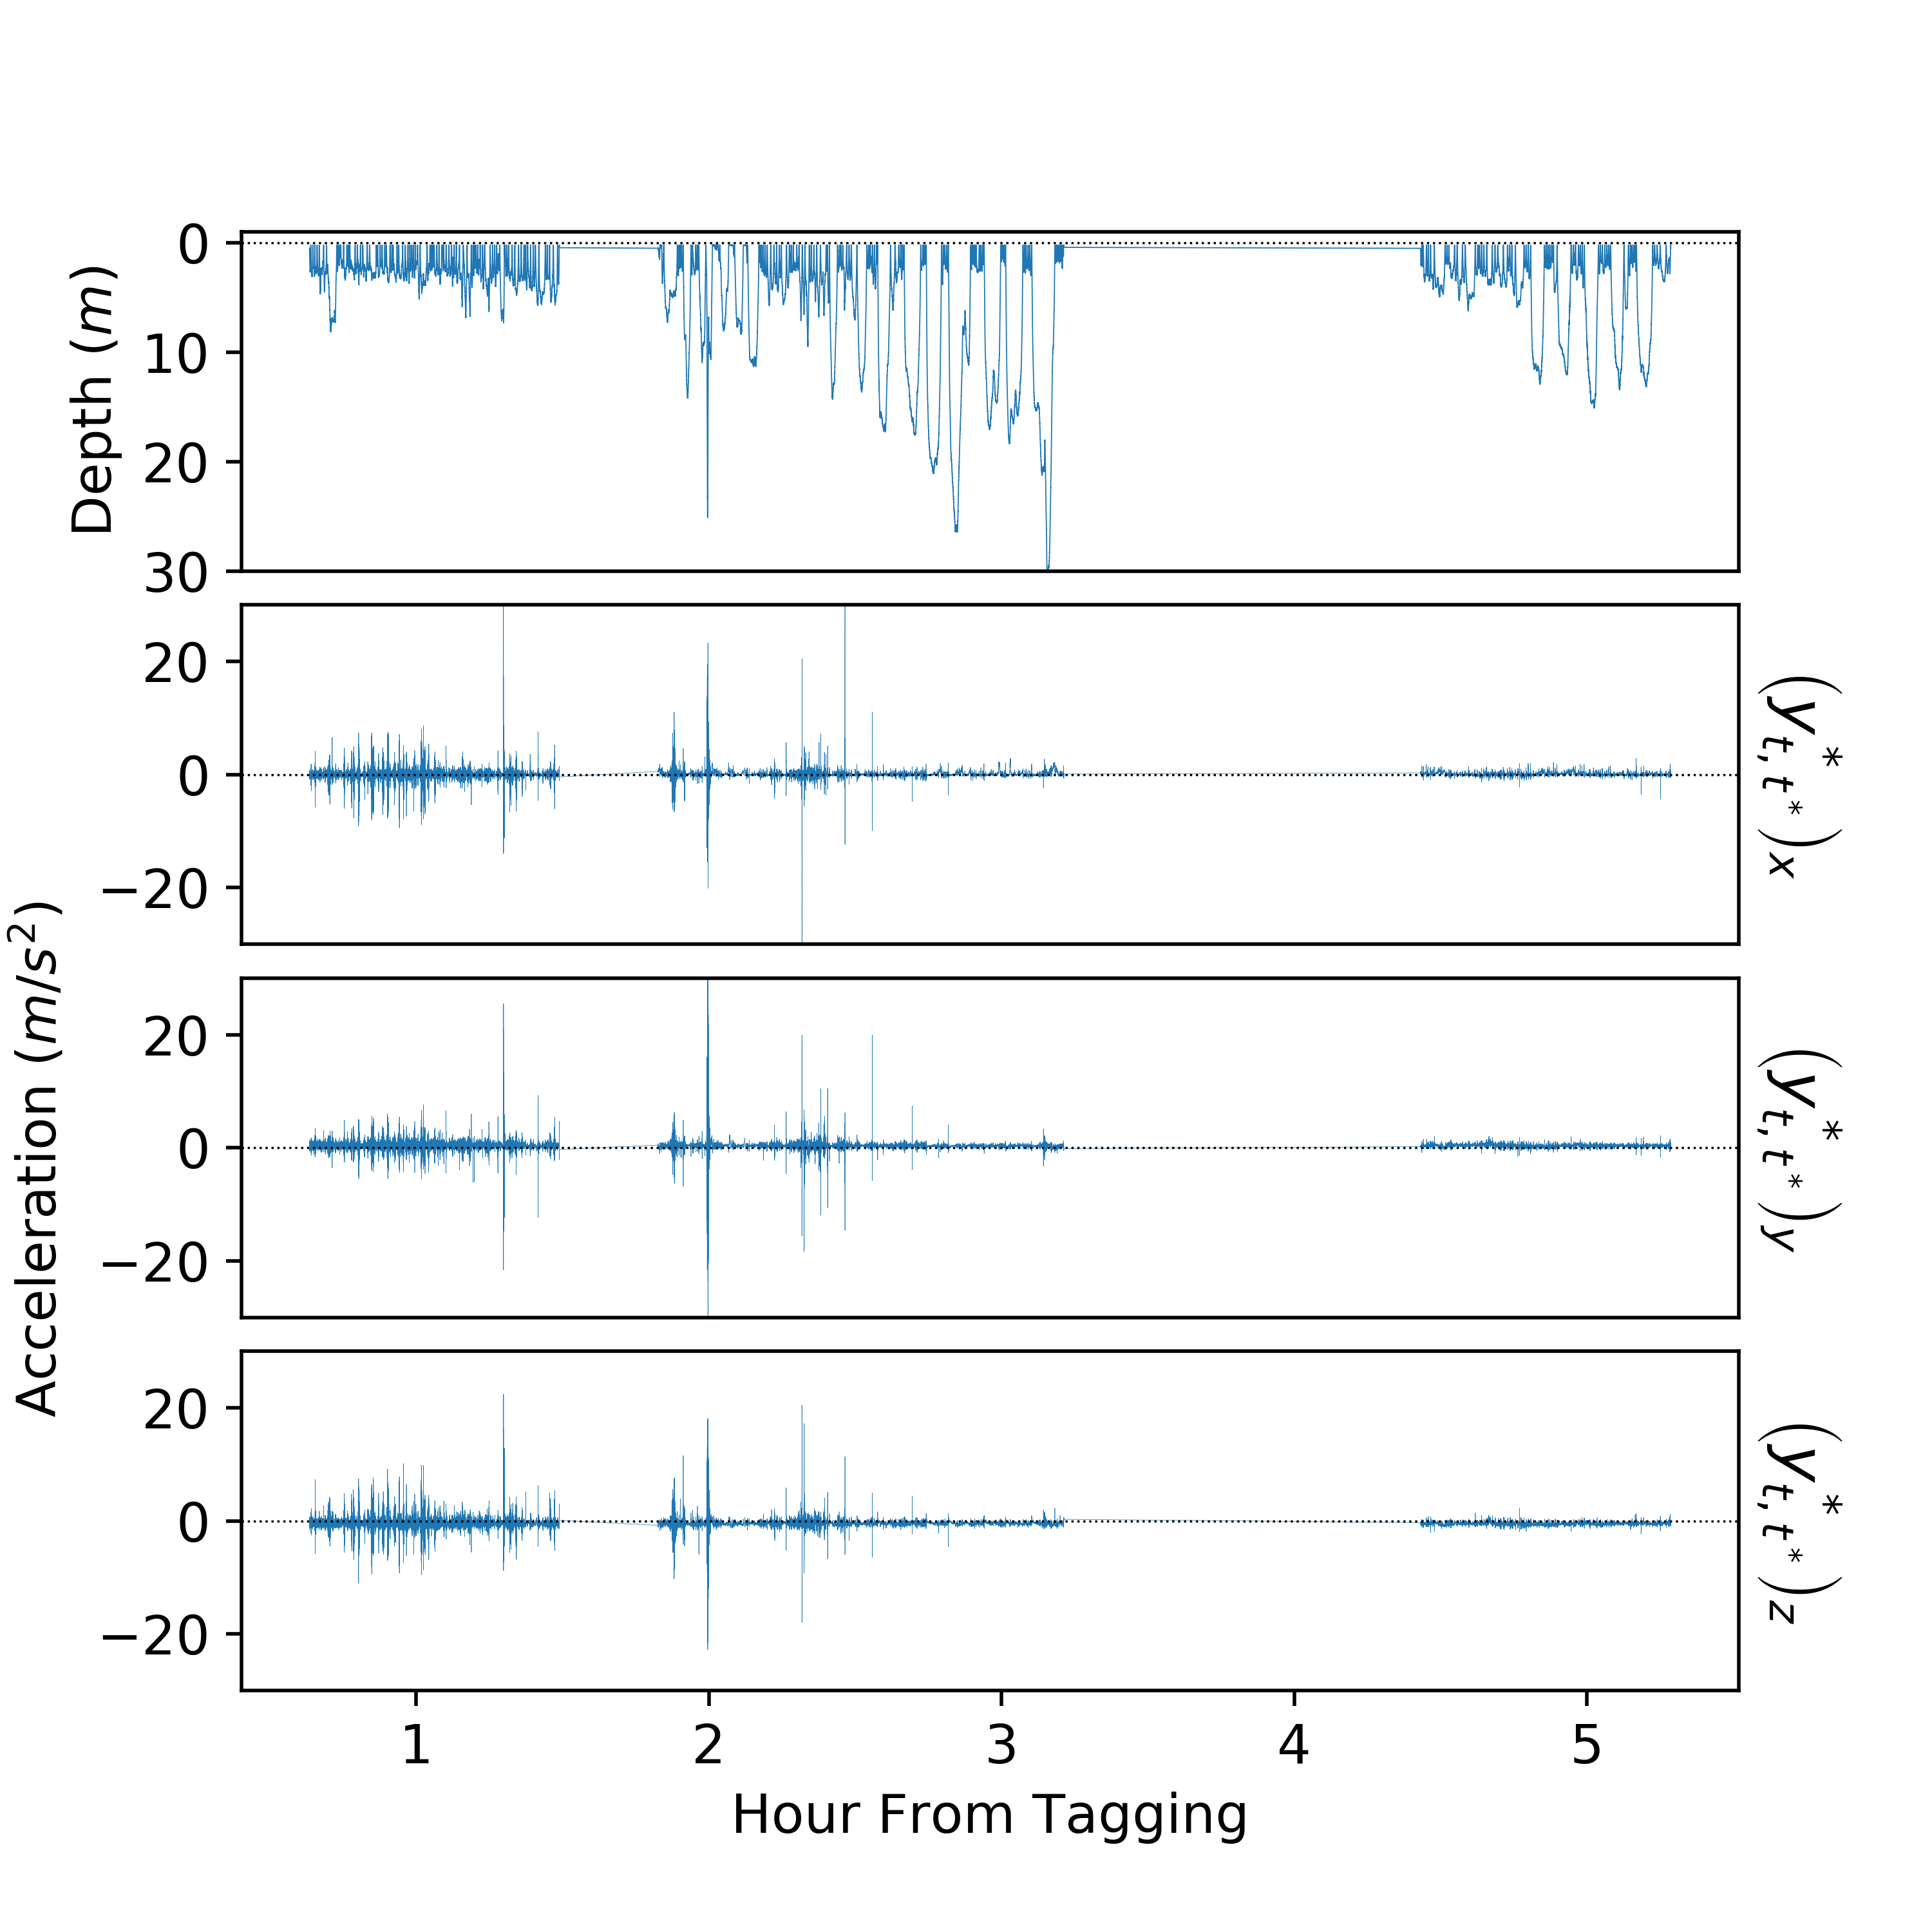
\includegraphics[width=5in]{../Plots/raw_data.png}
	\caption{Dive profile and Acceleration data of entire data set}
	\label{fig:data}
\end{figure}

\begin{figure}[ht]
	\centering
	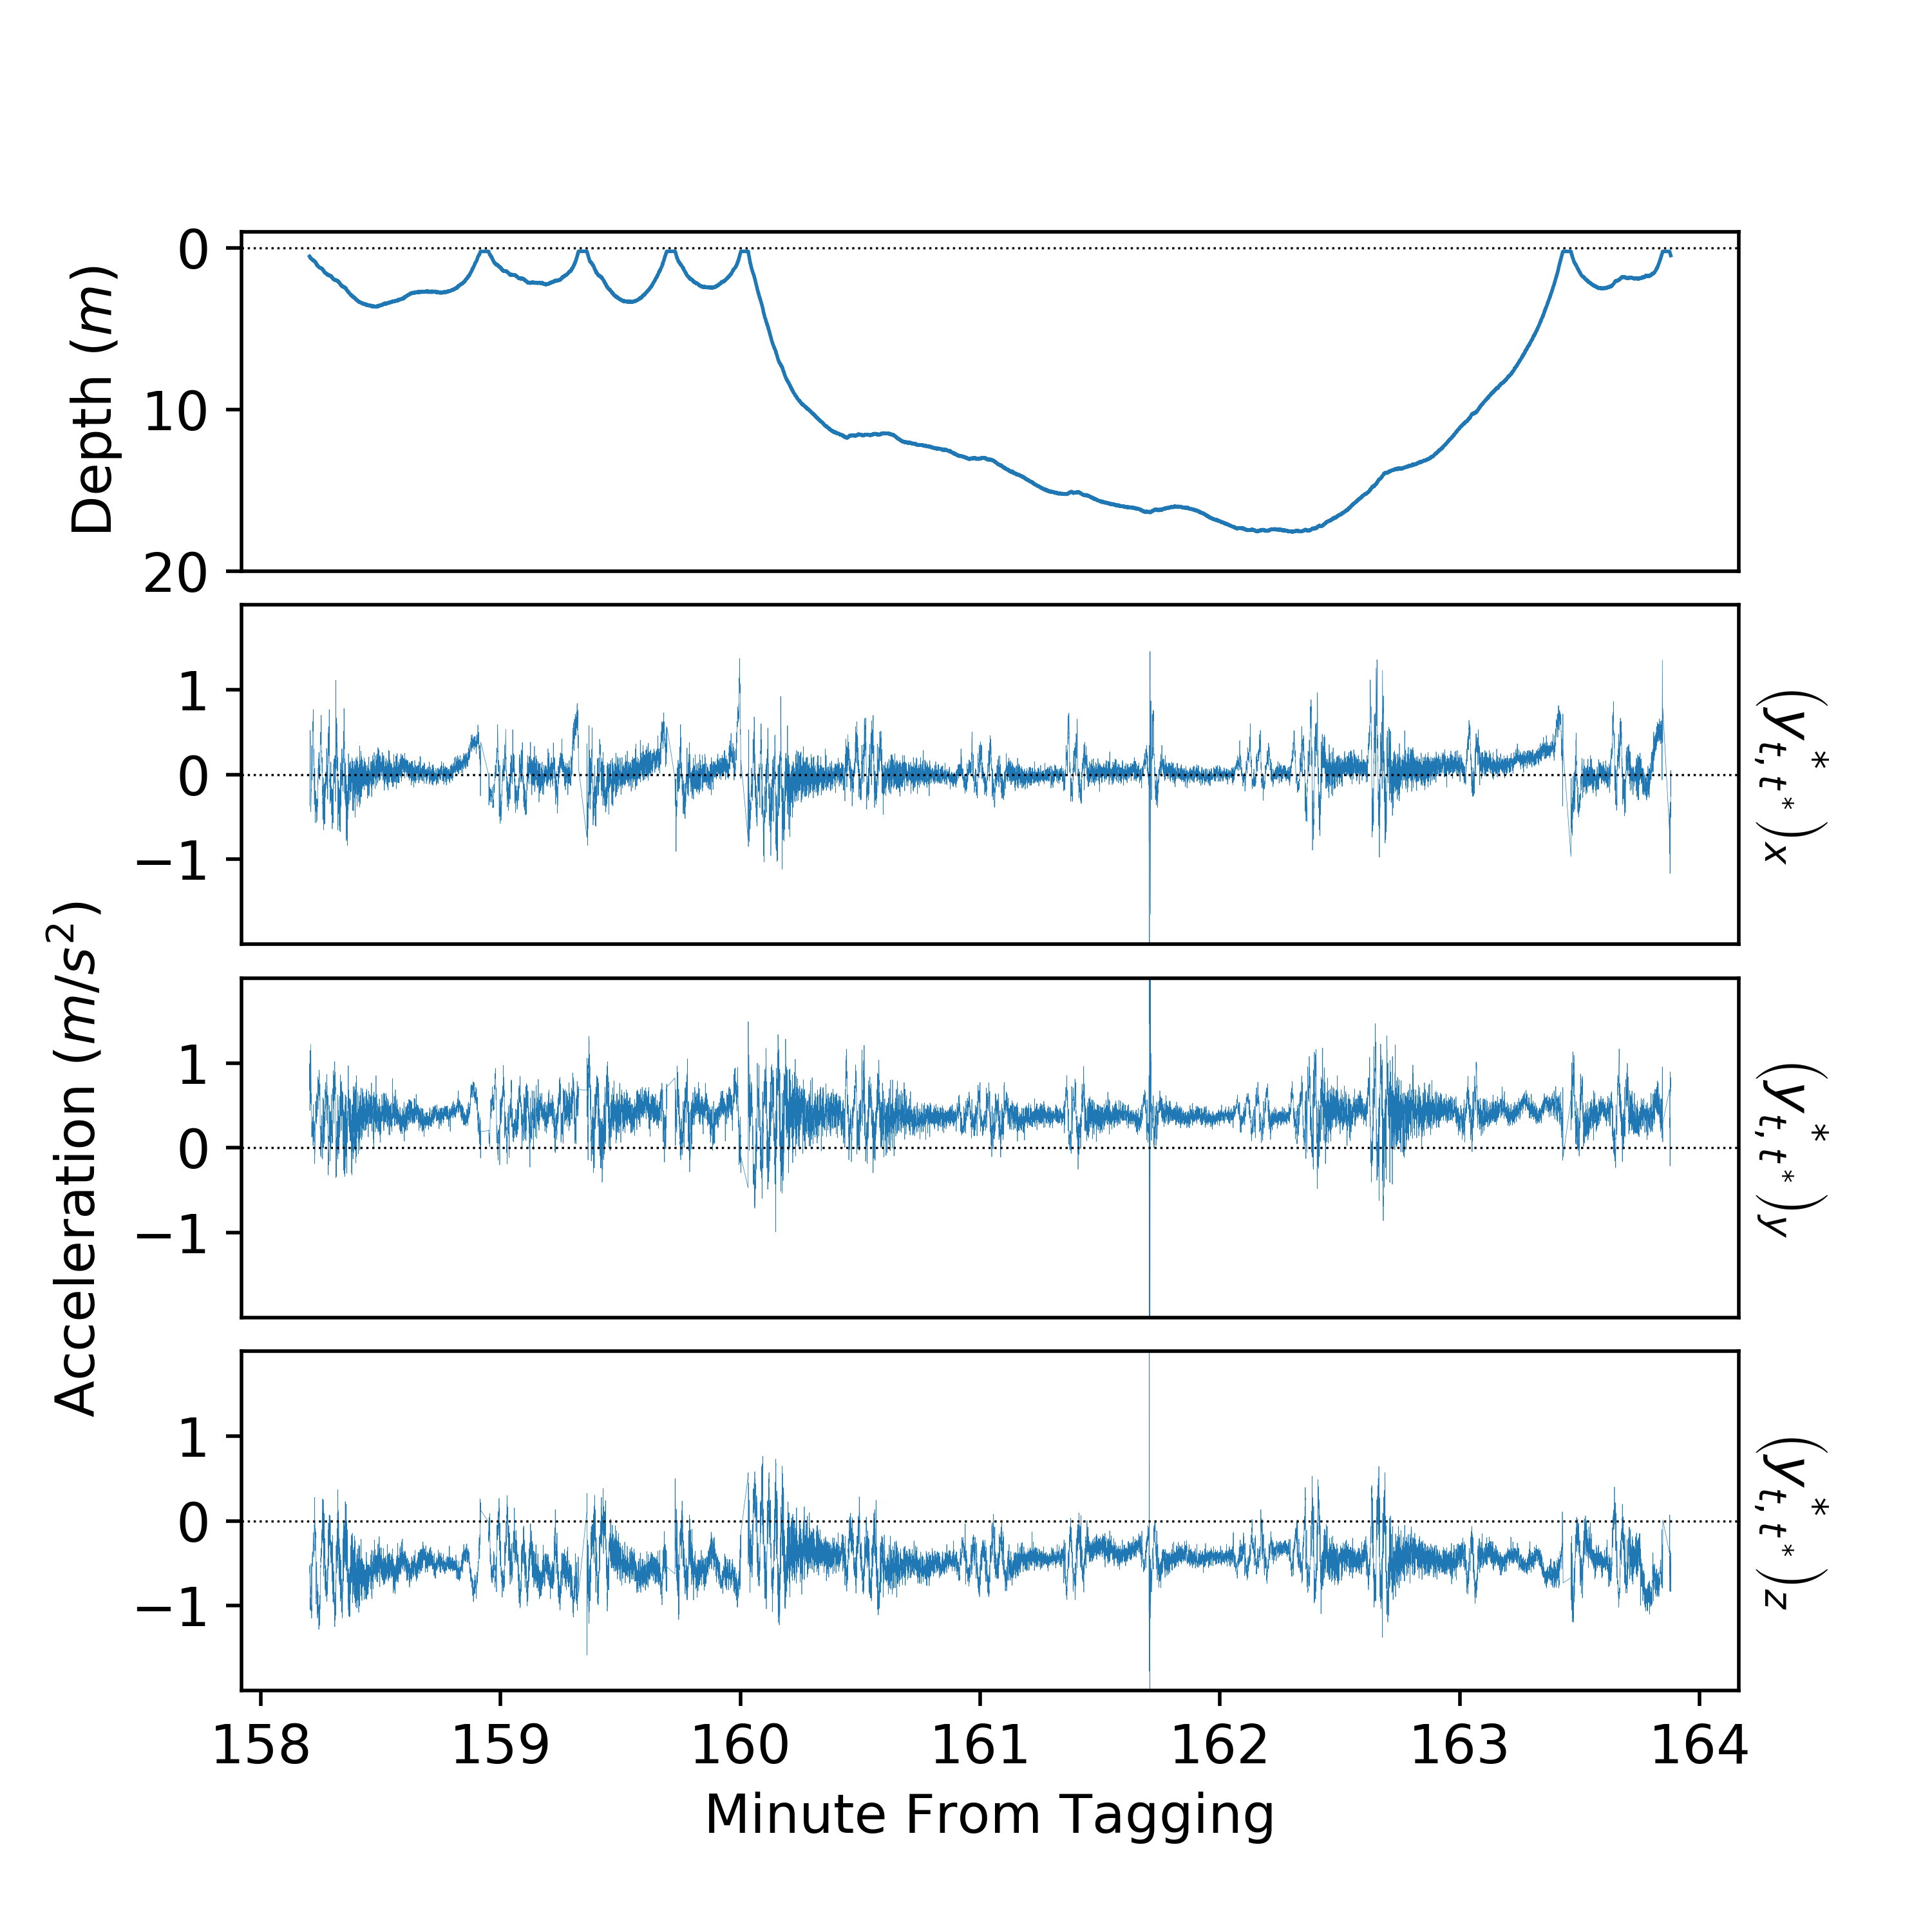
\includegraphics[width=5in]{../Plots/raw_data_5_dives.png}
	\caption{Dive profile and acceleration data for a collection of 5 dives of a killer whale.}
	\label{fig:data_one_dive}
\end{figure}

\begin{figure}[ht]
	\centering
	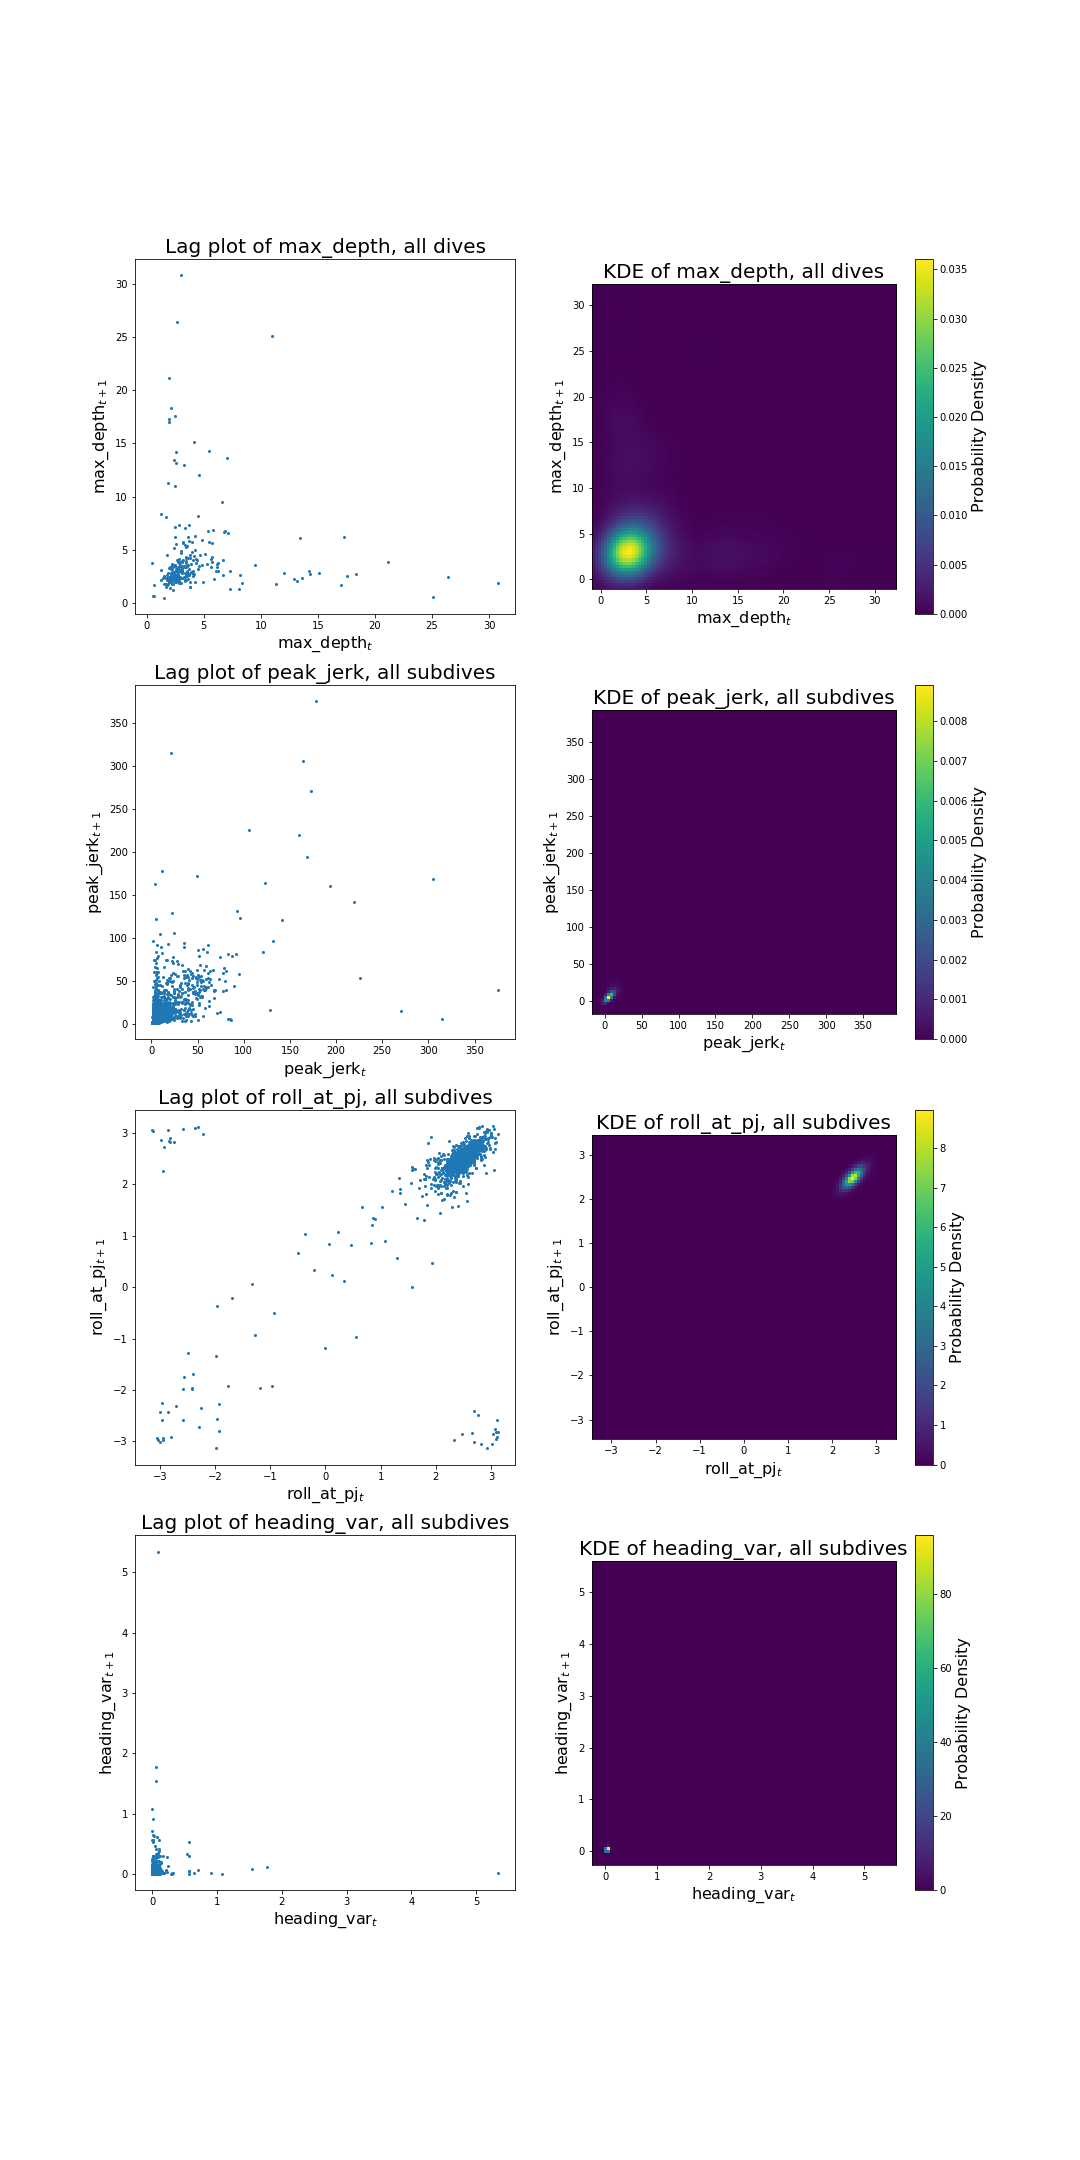
\includegraphics[height=7in]{../Plots/lagplot.png}
	\caption{Lag plots of all features on both the fine- and coarse- scale.}
	\label{fig:lag}
\end{figure}

\begin{figure}[ht]
	\centering
	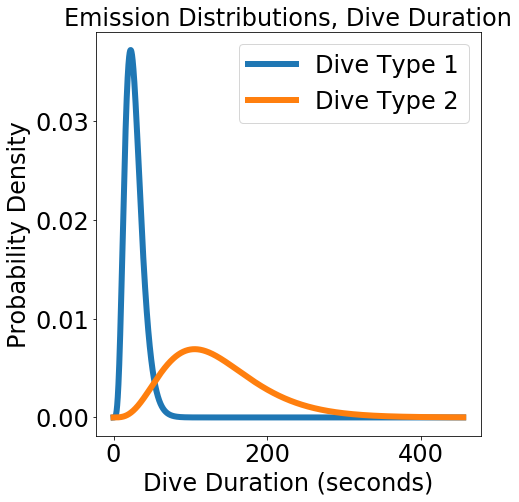
\includegraphics[width=5in]{../Plots/coarse-emissions.png}
	\caption{Estimated probability distributions for each coarse-scale observation in each dive type.}
	\label{fig:coarse_emis}
\end{figure}

\begin{figure}[ht]
	\centering
	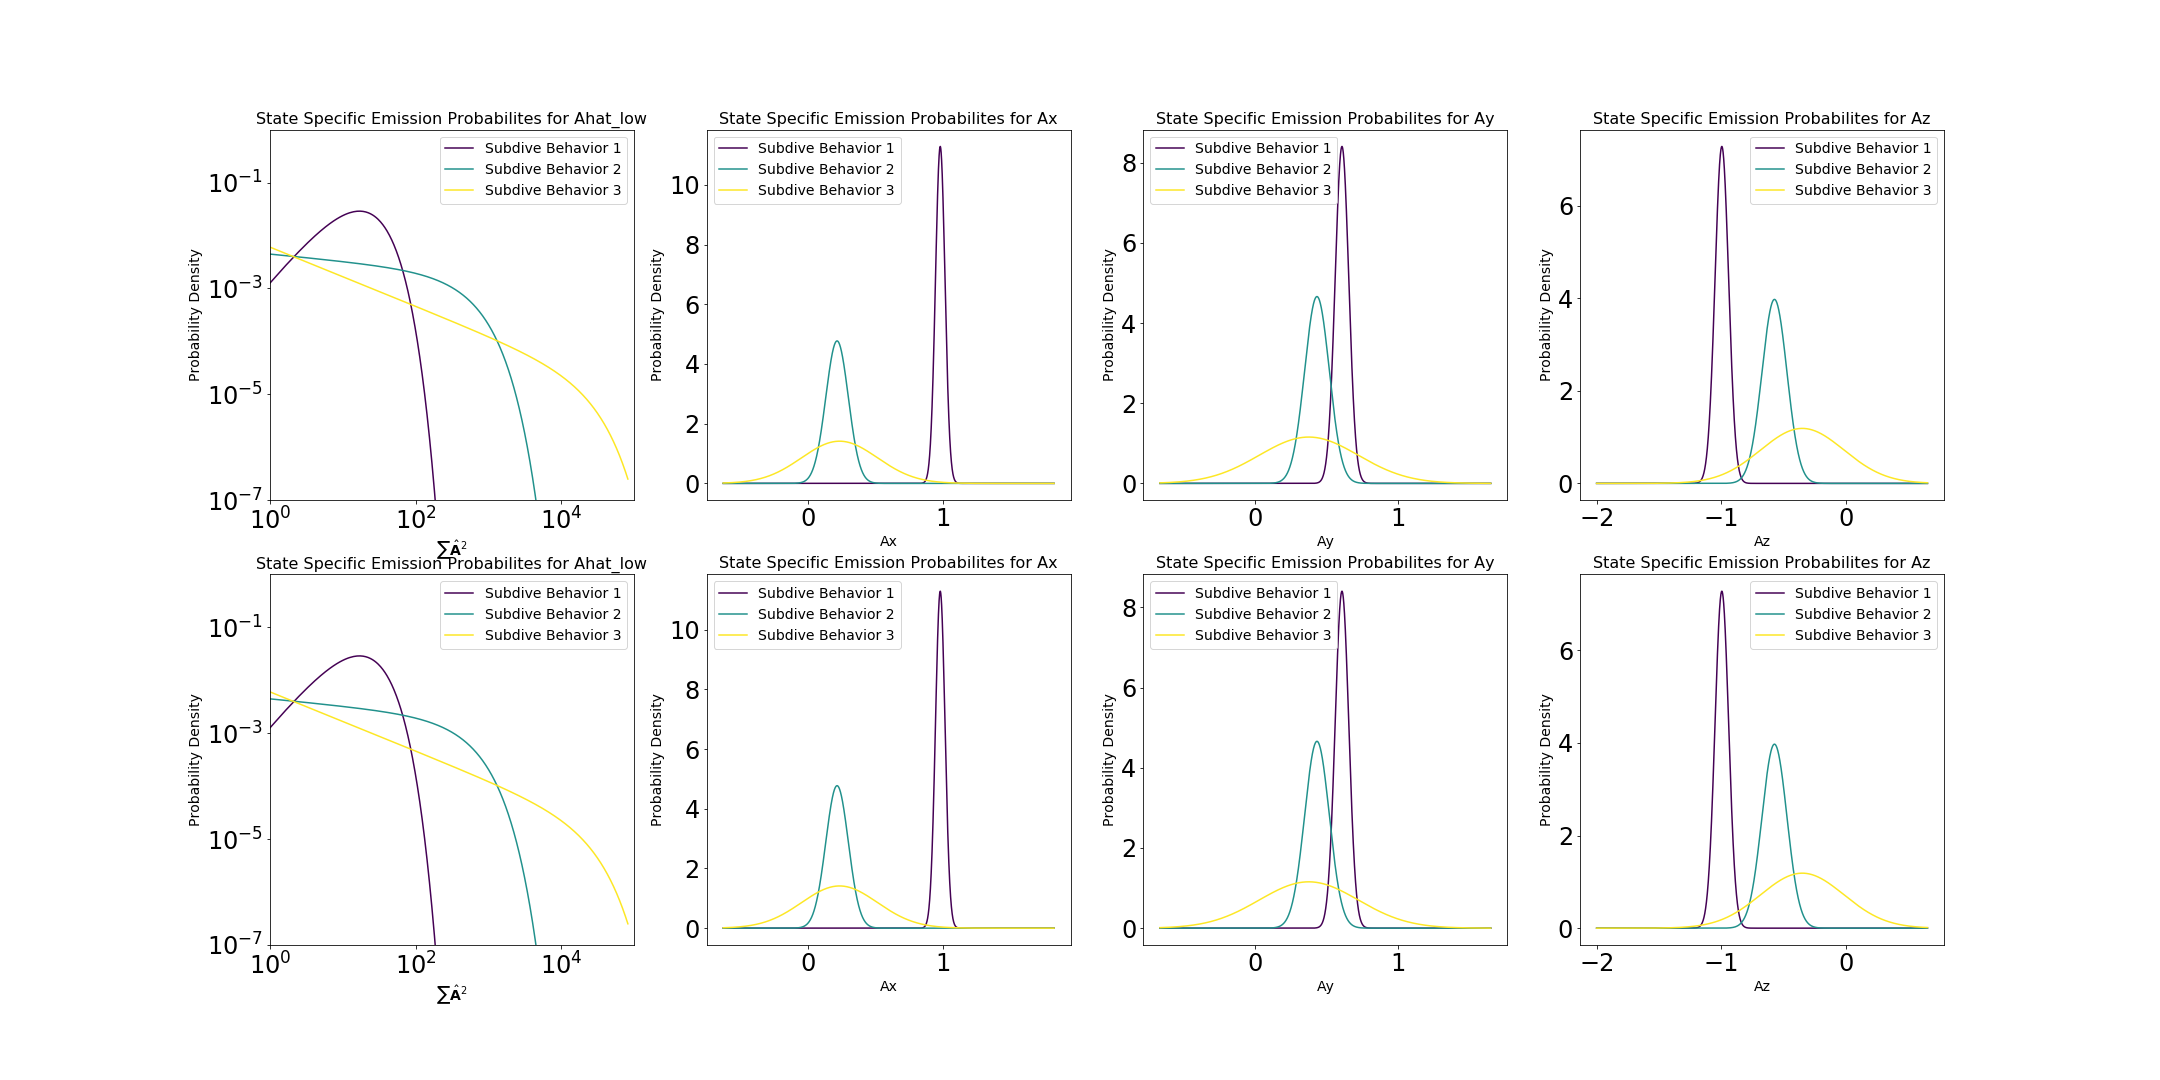
\includegraphics[width=5in]{../Plots/fine-emissions.png}
	\caption{Estimated probability distributions for each fine-scale observation in each behavioral state. Note that the distributions of acceleration do not take auto-correlation into account (see table \ref{table:emis_dists})}
	\label{fig:fine_emis}
\end{figure}

\begin{table}[ht]
    \centering
    \caption{Estimates and standard errors of emission parameters for killer whale data.}
    \scalebox{0.8}{
    \begin{tabular}{ccccc}
    \multirow{2}{*}{Feature}                 & \multirow{2}{*}{Dive / Sub-dive Type} & \multicolumn{3}{c}{Parameter Estimate}              \\
                                             &                                      & $\hat \mu$      & $\hat \sigma$   & $\hat \phi$     \\ \hline
    \multirow{2}{*}{Dive Duration (seconds)} & 1                                    & $27.23 \pm 0.63$ & $10.89 \pm 0.56$ & ---             \\
                                             & 2                                    & $127.96 \pm 11.50$ & $64.13 \pm 9.21$ & ---             \\ \hline
    \multirow{3}{*}{$Y^{*(1)}_x$}            & 1                                    & $0.98 \pm 0.07$ & $0.04 \pm 0.00$ & $0.99 \pm 0.00$ \\
                                             & 2                                    & $0.22 \pm 0.01$ & $0.08 \pm 0.00$ & $0.87 \pm 0.01$ \\
                                             & 3                                    & $0.23 \pm 0.03$ & $0.28 \pm 0.01$ & $0.62 \pm 0.03$ \\ \hline
    \multirow{3}{*}{$Y^{*(1)}_y$}            & 1                                    & $0.61 \pm 0.09$ & $0.05 \pm 0.00$ & $0.99 \pm 0.00$ \\
                                             & 2                                    & $0.43 \pm 0.01$ & $0.09 \pm 0.00$ & $0.87 \pm 0.01$ \\
                                             & 3                                    & $0.38 \pm 0.04$ & $0.35 \pm 0.01$ & $0.62 \pm 0.04$ \\ \hline
    \multirow{3}{*}{$Y^{*(1)}_z$}            & 1                                    & $-1.00 \pm 0.11$ & $0.05 \pm 0.00$ & $0.99 \pm 0.00$ \\
                                             & 2                                    & $-0.57 \pm 0.01$ & $0.10 \pm 0.00$ & $0.87 \pm 0.01$ \\
                                             & 3                                    & $-0.35 \pm 0.04$ & $0.34 \pm 0.01$ & $0.62 \pm 0.04$ \\ \hline
    \multirow{3}{*}{$Y^{*(2)}$}              & 1                                    & $27.16 \pm 0.32$ & $16.67 \pm 0.32$ & ---             \\
                                             & 2                                    & $406.98 \pm 4.42$ & $438.09 \pm 5.49$ & ---             \\
                                             & 3                                    & $9688.54 \pm 221.95$ & $14584.02 \pm 358.40$ & ---             \\ \hline
    \end{tabular}
    }
    \label{table:emis_dists}
\end{table}

\begin{figure}[ht]
	\centering
	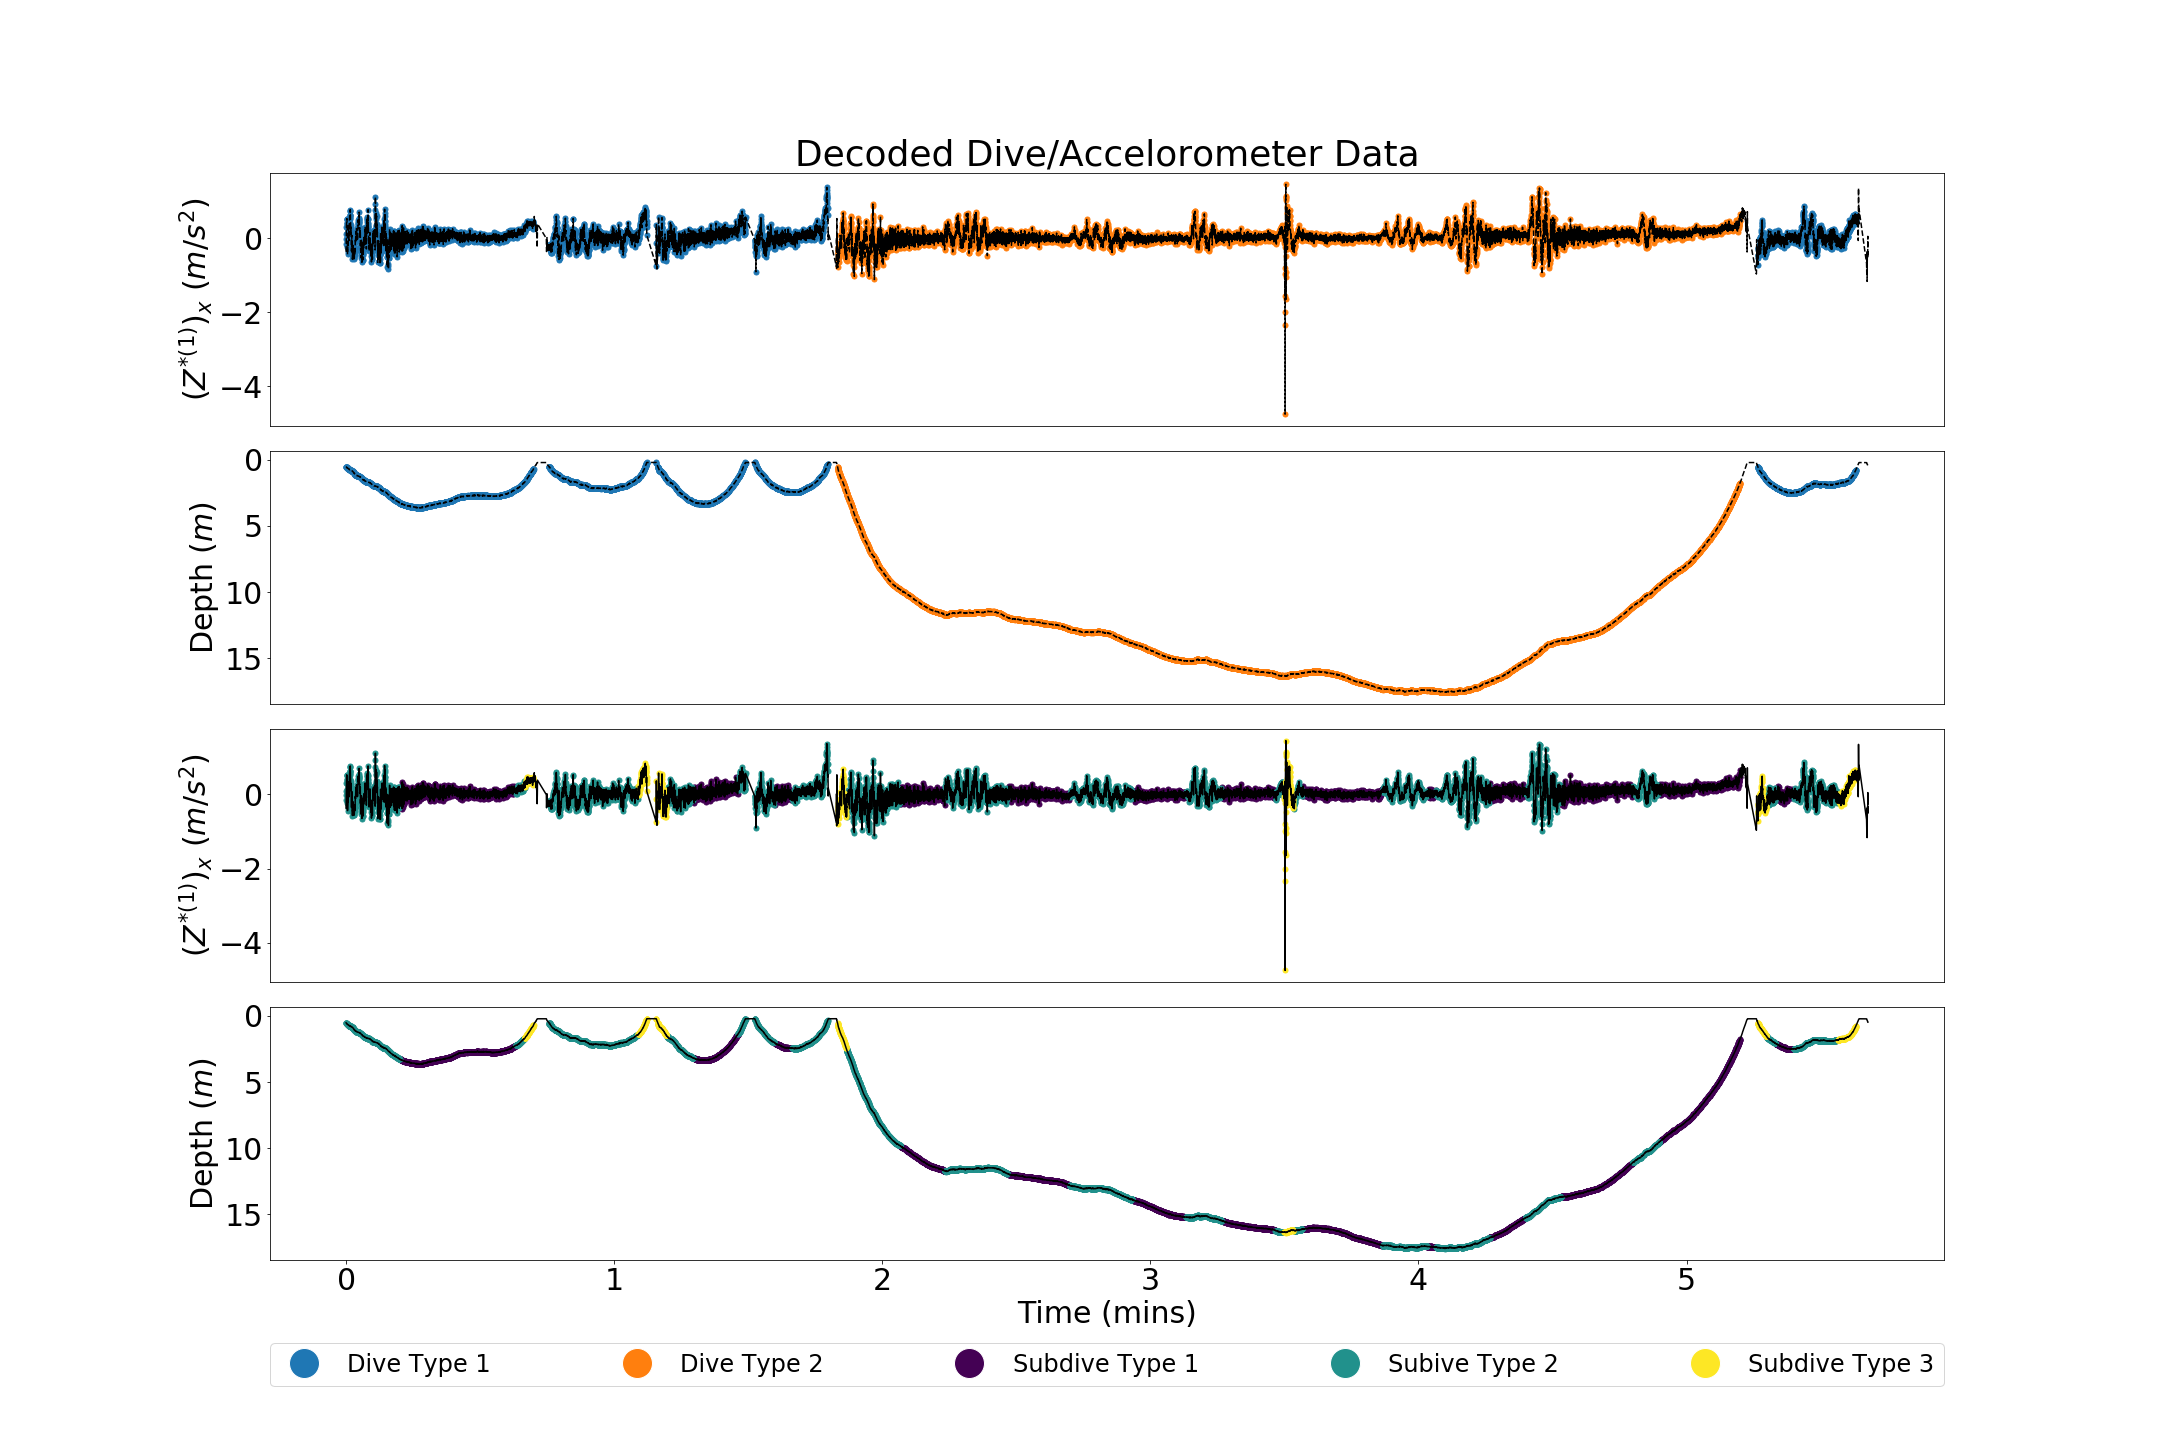
\includegraphics[width=5in]{../Plots/decoded_data.png}
	\caption{Features of a particular set of killer whale dives and decoded estimates for the intra-dive behavioral states. The color of the plot corresponds to behavioral or dive state with the highest probability.}
	\label{fig:labeled_dives}
\end{figure}
%
\begin{figure}[ht]
	\centering
	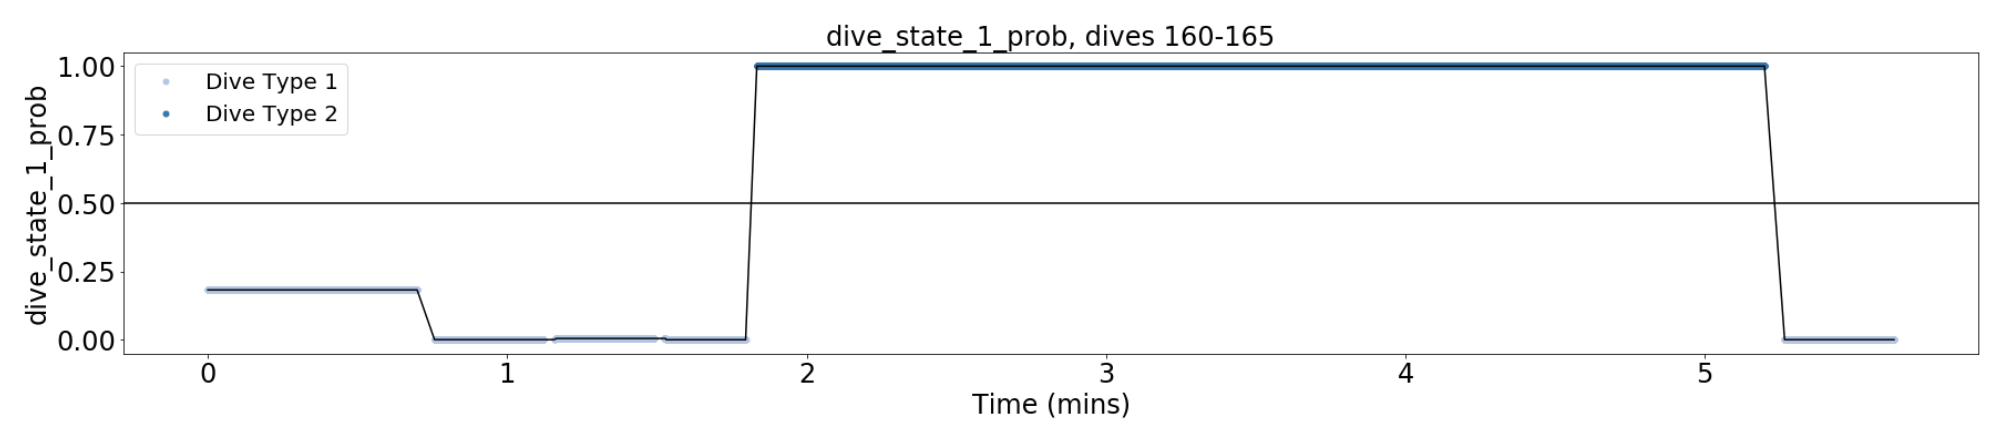
\includegraphics[width=5in]{../Plots/Coarse_state_probs.png}
	\caption{Probabilities of dive types for the set of killer whale dives from (fig \ref{fig:labeled_dives}).}
	\label{fig:coarse_probs}
\end{figure}
%
\begin{figure}[ht]
	\centering
	\begin{subfigure}[t]{1.0\textwidth}
        \centering
        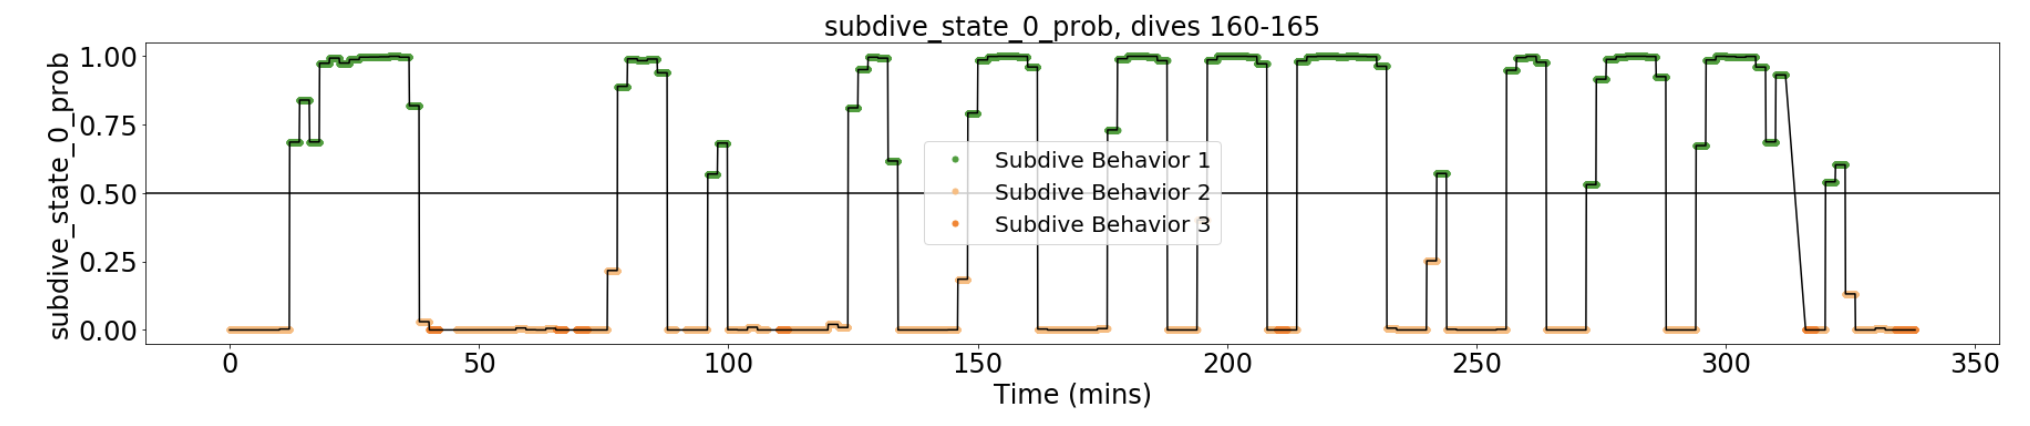
\includegraphics[width=5in]{../Plots/Fine_state_probs_1.png}
        \caption{Fine-scale state 1 probabilities}
    \end{subfigure}
    \newline
    \begin{subfigure}[t]{1.0\textwidth}
        \centering
        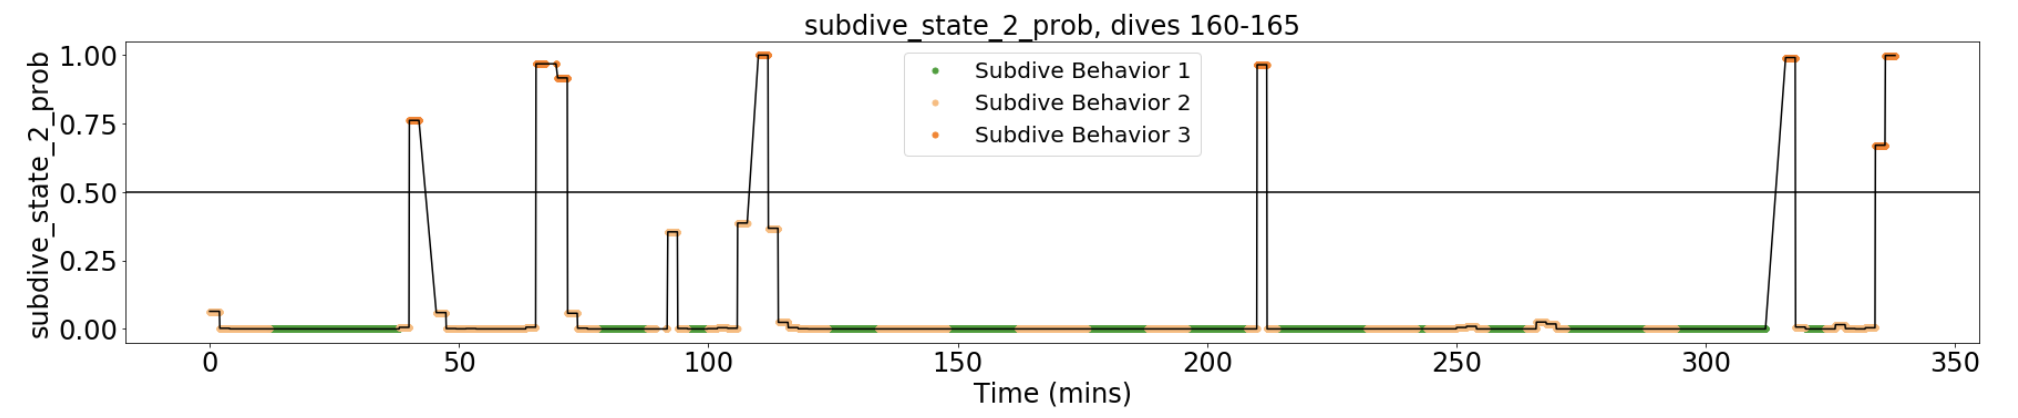
\includegraphics[width=5in]{../Plots/Fine_state_probs_3.png}
        \caption{Fine-scale state 3 probabilities}
    \end{subfigure}
	\caption{Probabilities of sub-dive types for the set of killer whale dives from (fig \ref{fig:labeled_dives}).}
	\label{fig:fine_probs}
\end{figure}

\begin{figure}[ht]
	\centering
	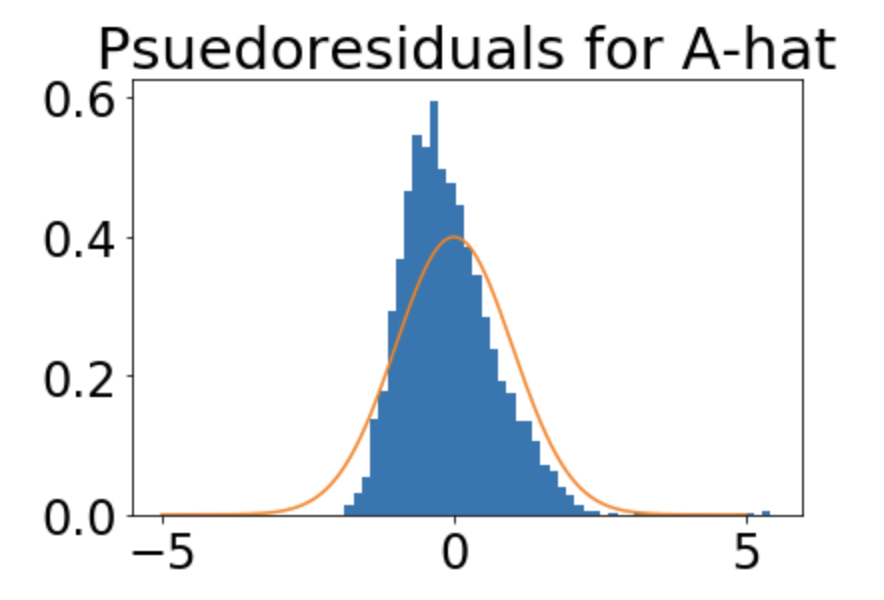
\includegraphics[width=5in]{../Plots/pseudoresids.png}
	\caption{Psuedoresiduals of $Y^{*(2)}$}
	\label{fig:pseudoresids}
\end{figure}

\begin{figure}[ht]
	\centering
	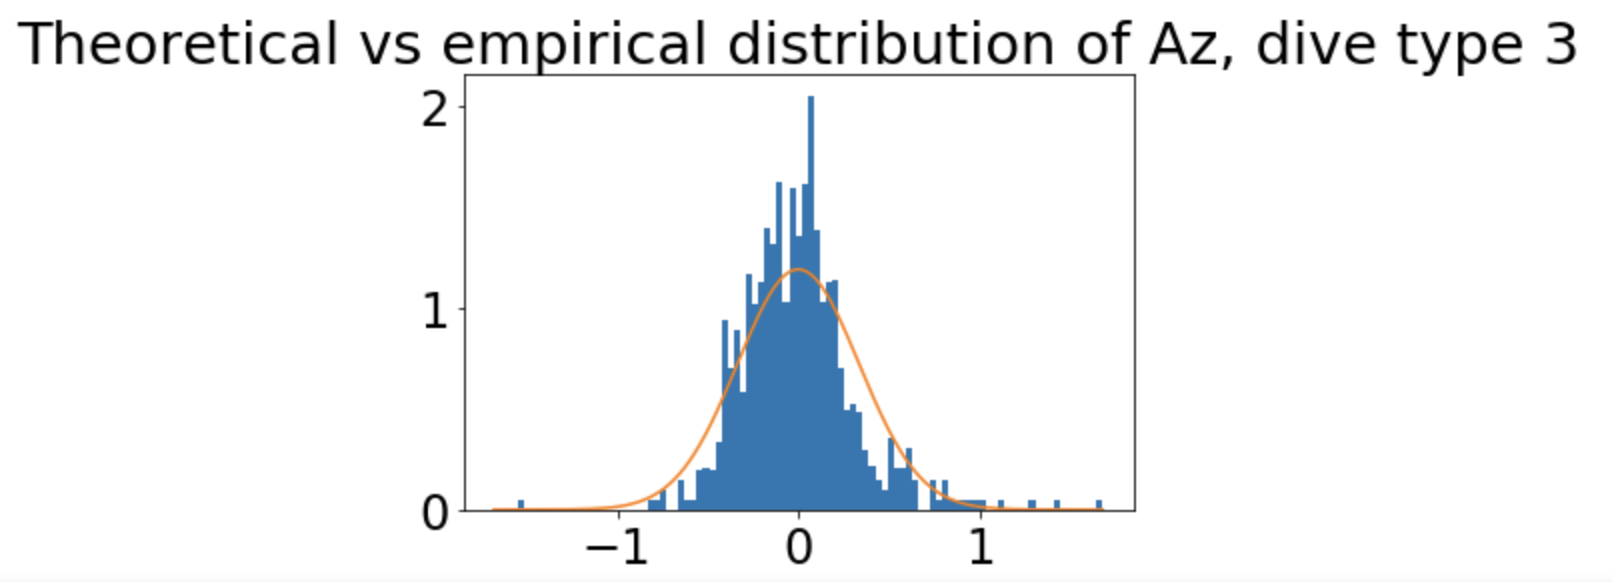
\includegraphics[width=5in]{../Plots/empirical_dist.png}
	\caption{Empirical distribution of $Y^{*(1)}_z$ for sub-dive state 3 plotted over its estimated pdf.}
	\label{fig:empirical_dist}
\end{figure}